\documentclass[11pt]{article}
\usepackage[textwidth=18.0cm, textheight=23.0cm, top=2.0cm]{geometry}
\usepackage{pst-all}
\usepackage{amssymb}
\usepackage{tikz}
\usepackage{underscore}\begin{document}
\pagestyle{empty}


ClassName: \underline{\textbf{Class_03.2bp-49}}
\par
BinSize: \underline{\textbf{40 × 40}}
\par
ReduceSize: \underline{\textbf{40 × 40}}
\par
TypeNum: \underline{\textbf{99}}
\par
Num: \underline{\textbf{100}}
\par
OutS: \underline{\textbf{46400}}
\par
InS: \underline{\textbf{37188}}
\par
Rate: \underline{\textbf{0.801}}
\par
UB: \underline{\textbf{29}}
\par
LB0: \underline{\textbf{29}}
\par
LB: \underline{\textbf{29}}
\par
LBWithCut: \underline{\textbf{29}}
\par
NodeCut: \underline{\textbf{0}}
\par
ExtendedNodeCnt: \underline{\textbf{1}}
\par
GenNodeCnt: \underline{\textbf{1}}
\par
PrimalNode: \underline{\textbf{0}}
\par
ColumnCount: \underline{\textbf{29}}
\par
TotalCutCount: \underline{\textbf{0}}
\par
RootCutCount: \underline{\textbf{0}}
\par
LPSolverCnt: \underline{\textbf{1}}
\par
PricingSolverCnt: \underline{\textbf{0}}
\par
BranchAndBoundNum: \underline{\textbf{1}}
\par
isOpt: \underline{\textbf{true}}
\par
TimeOnInitSolution: \underline{\textbf{600.000 s}}
\par
TimeOnPrimal: \underline{\textbf{0.000 s}}
\par
TimeOnPricing: \underline{\textbf{0.000 s}}
\par
TimeOnRmp: \underline{\textbf{0.066 s}}
\par
TotalTime: \underline{\textbf{600.362 s}}
\par
\newpage


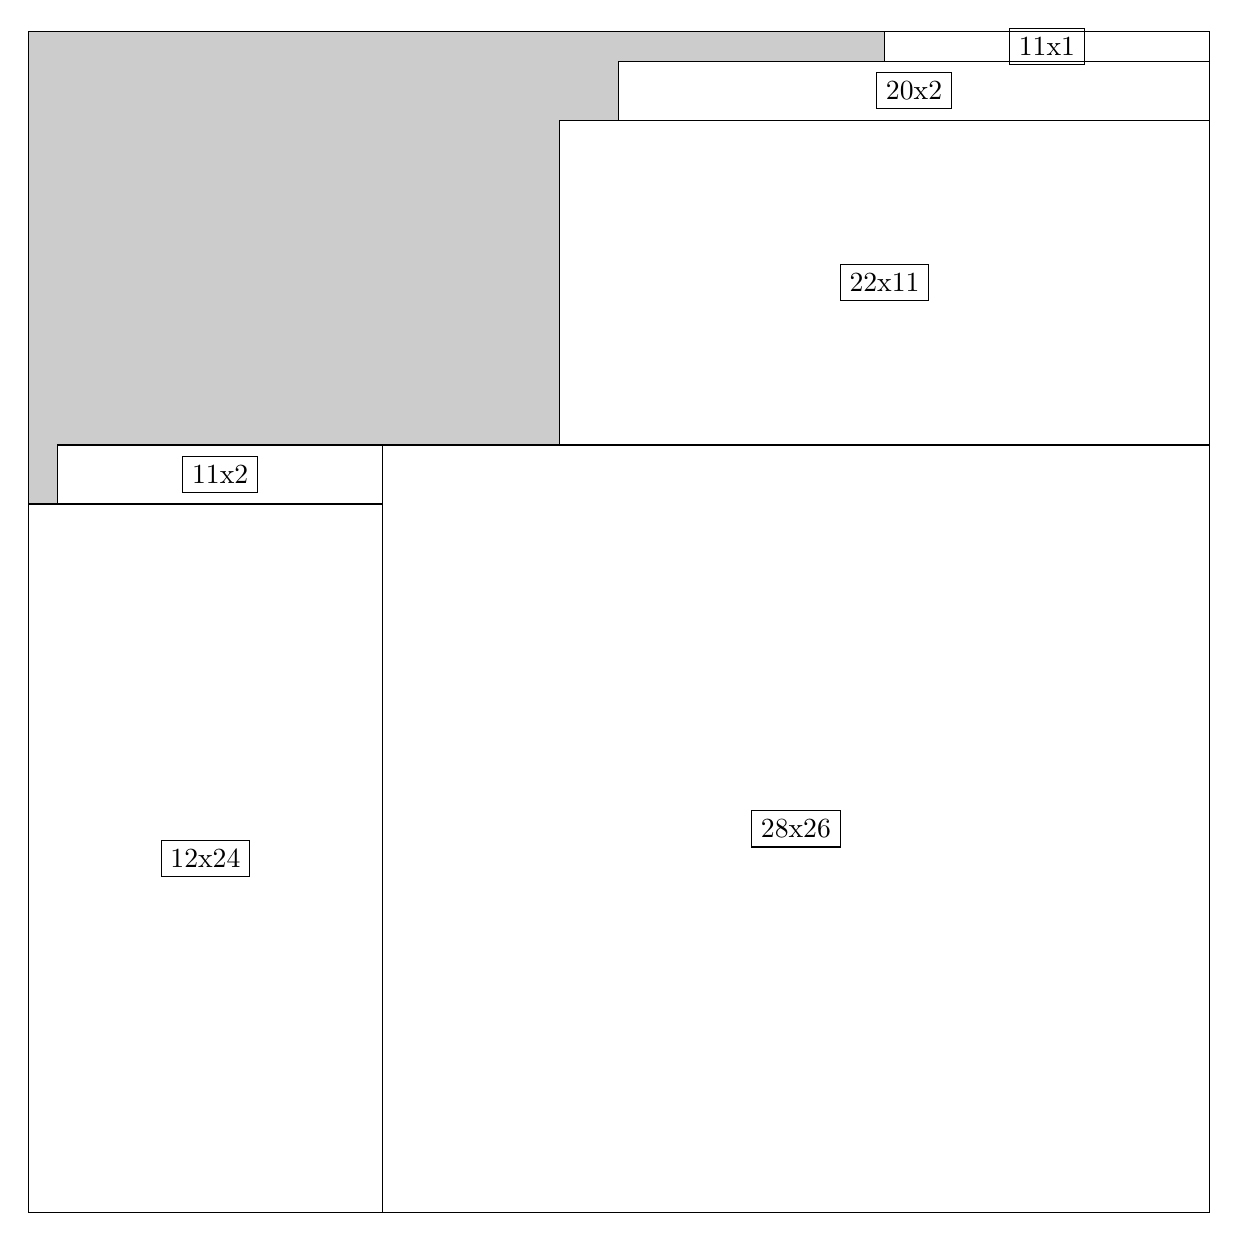
\begin{tikzpicture}[shorten >=1pt,scale=1.0,every node/.style={scale=1.0},->]
\tikzstyle{vertex}=[circle,fill=black!25,minimum size=14pt,inner sep=0pt]
\filldraw[fill=gray!40!white, draw=black] (0,0) rectangle (15.0,15.0);
\foreach \name/\x/\y/\w/\h in {28x26/4.5/0.0/10.5/9.75,12x24/0.0/0.0/4.5/9.0,11x2/0.375/9.0/4.125/0.75,22x11/6.75/9.75/8.25/4.125,20x2/7.5/13.875/7.5/0.75,11x1/10.875/14.625/4.125/0.375}
\filldraw[fill=white!40!white, draw=black] (\x,\y) rectangle node[draw] (\name) {\name} ++(\w,\h);
\end{tikzpicture}


w =28 , h =26 , x =12 , y =0 , v =728
\par
w =12 , h =24 , x =0 , y =0 , v =288
\par
w =11 , h =2 , x =1 , y =24 , v =22
\par
w =22 , h =11 , x =18 , y =26 , v =242
\par
w =20 , h =2 , x =20 , y =37 , v =40
\par
w =11 , h =1 , x =29 , y =39 , v =11
\par
\newpage


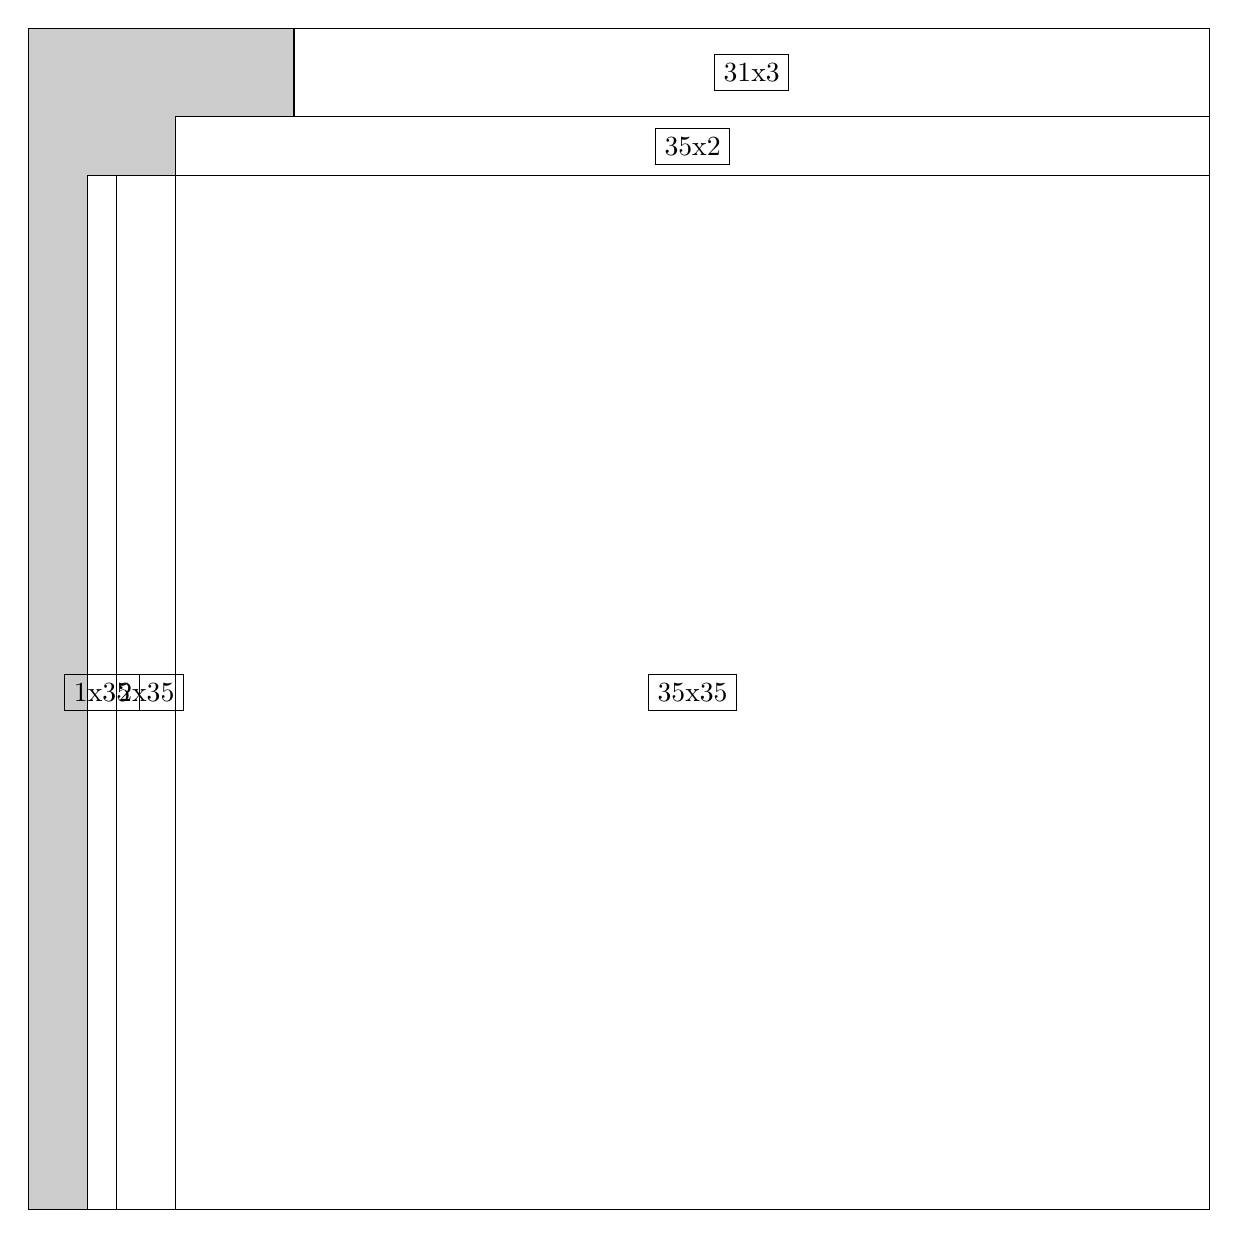
\begin{tikzpicture}[shorten >=1pt,scale=1.0,every node/.style={scale=1.0},->]
\tikzstyle{vertex}=[circle,fill=black!25,minimum size=14pt,inner sep=0pt]
\filldraw[fill=gray!40!white, draw=black] (0,0) rectangle (15.0,15.0);
\foreach \name/\x/\y/\w/\h in {35x35/1.875/0.0/13.125/13.125,35x2/1.875/13.125/13.125/0.75,31x3/3.375/13.875/11.625/1.125,2x35/1.125/0.0/0.75/13.125,1x35/0.75/0.0/0.375/13.125}
\filldraw[fill=white!40!white, draw=black] (\x,\y) rectangle node[draw] (\name) {\name} ++(\w,\h);
\end{tikzpicture}


w =35 , h =35 , x =5 , y =0 , v =1225
\par
w =35 , h =2 , x =5 , y =35 , v =70
\par
w =31 , h =3 , x =9 , y =37 , v =93
\par
w =2 , h =35 , x =3 , y =0 , v =70
\par
w =1 , h =35 , x =2 , y =0 , v =35
\par
\newpage


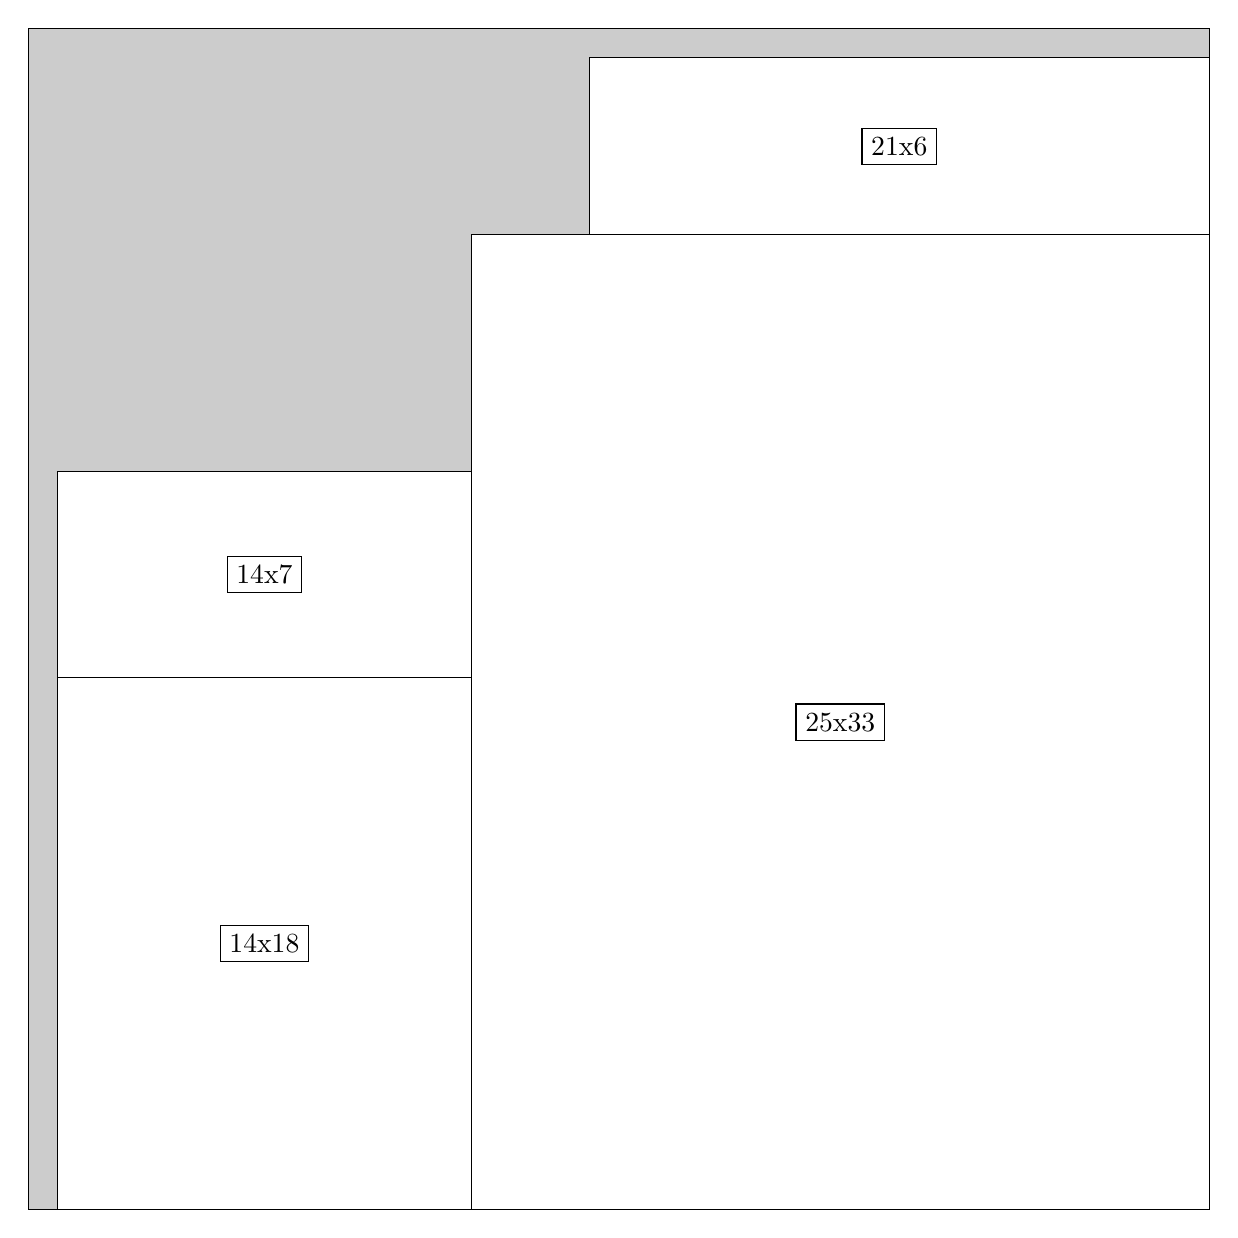
\begin{tikzpicture}[shorten >=1pt,scale=1.0,every node/.style={scale=1.0},->]
\tikzstyle{vertex}=[circle,fill=black!25,minimum size=14pt,inner sep=0pt]
\filldraw[fill=gray!40!white, draw=black] (0,0) rectangle (15.0,15.0);
\foreach \name/\x/\y/\w/\h in {25x33/5.625/0.0/9.375/12.375,21x6/7.125/12.375/7.875/2.25,14x18/0.375/0.0/5.25/6.75,14x7/0.375/6.75/5.25/2.625}
\filldraw[fill=white!40!white, draw=black] (\x,\y) rectangle node[draw] (\name) {\name} ++(\w,\h);
\end{tikzpicture}


w =25 , h =33 , x =15 , y =0 , v =825
\par
w =21 , h =6 , x =19 , y =33 , v =126
\par
w =14 , h =18 , x =1 , y =0 , v =252
\par
w =14 , h =7 , x =1 , y =18 , v =98
\par
\newpage


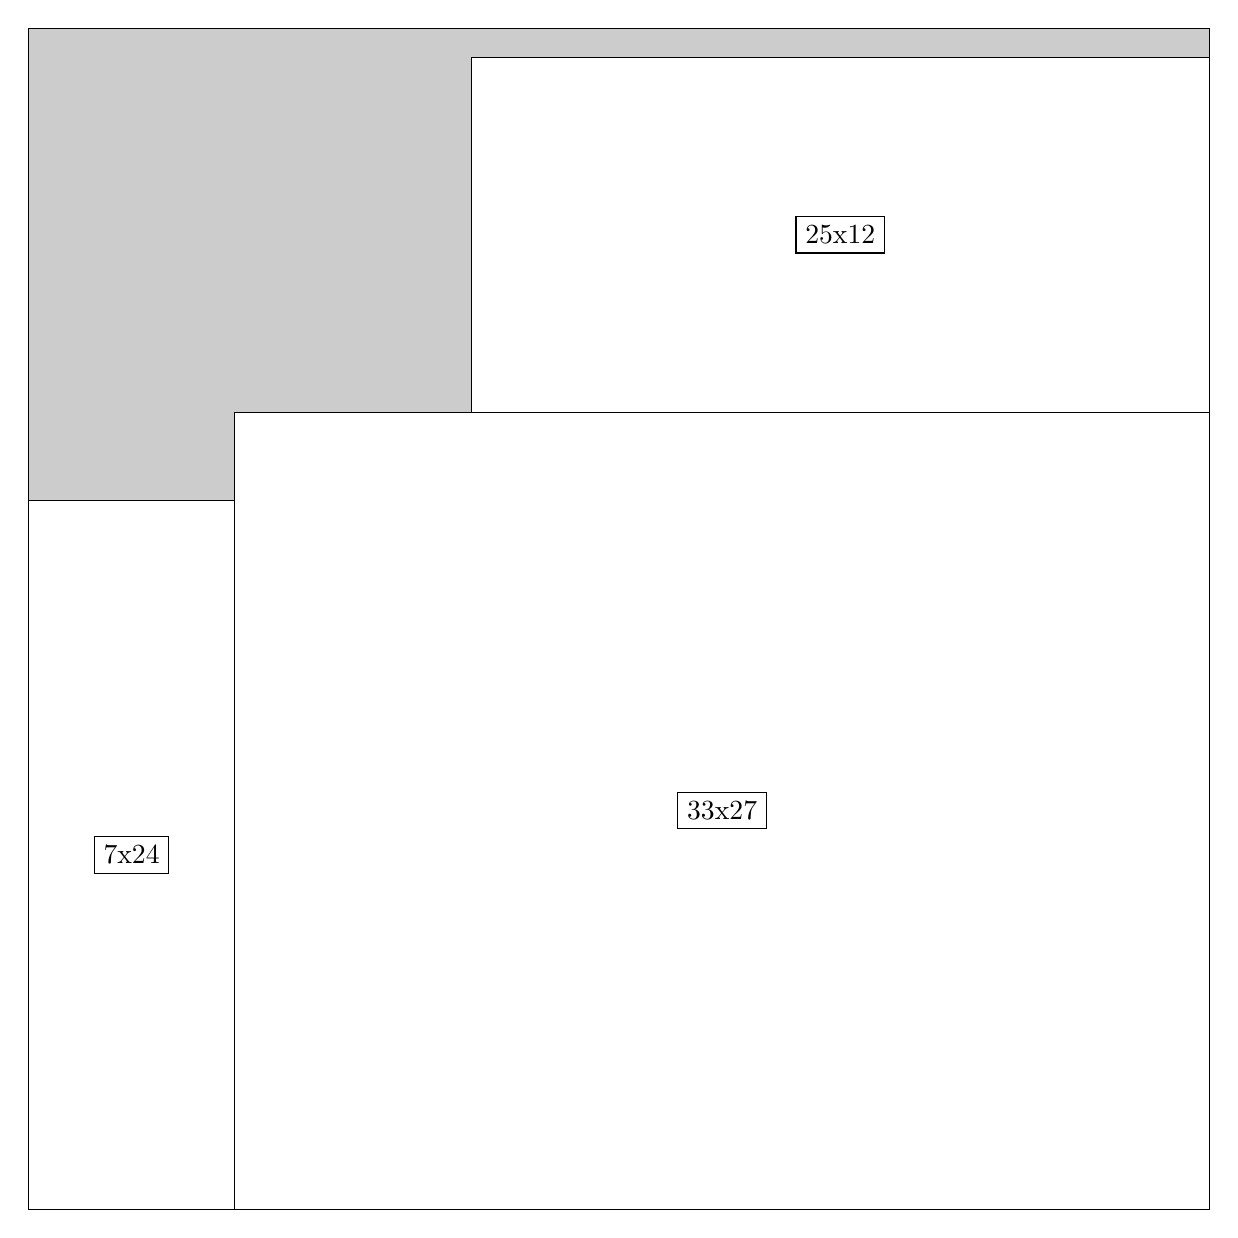
\begin{tikzpicture}[shorten >=1pt,scale=1.0,every node/.style={scale=1.0},->]
\tikzstyle{vertex}=[circle,fill=black!25,minimum size=14pt,inner sep=0pt]
\filldraw[fill=gray!40!white, draw=black] (0,0) rectangle (15.0,15.0);
\foreach \name/\x/\y/\w/\h in {33x27/2.625/0.0/12.375/10.125,25x12/5.625/10.125/9.375/4.5,7x24/0.0/0.0/2.625/9.0}
\filldraw[fill=white!40!white, draw=black] (\x,\y) rectangle node[draw] (\name) {\name} ++(\w,\h);
\end{tikzpicture}


w =33 , h =27 , x =7 , y =0 , v =891
\par
w =25 , h =12 , x =15 , y =27 , v =300
\par
w =7 , h =24 , x =0 , y =0 , v =168
\par
\newpage


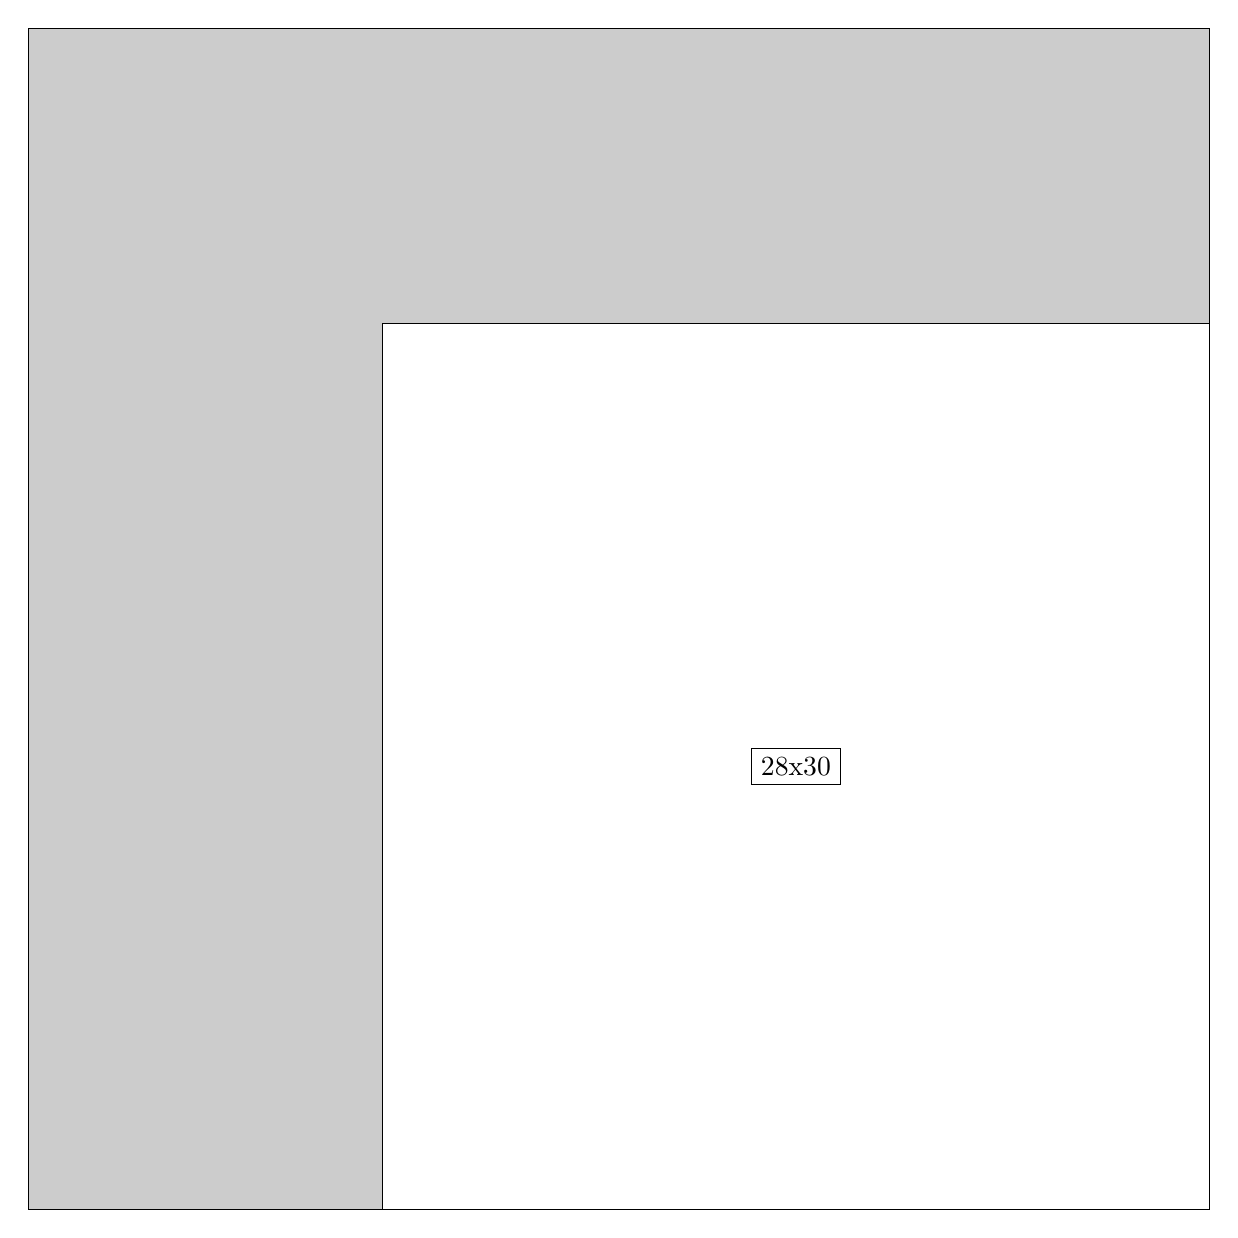
\begin{tikzpicture}[shorten >=1pt,scale=1.0,every node/.style={scale=1.0},->]
\tikzstyle{vertex}=[circle,fill=black!25,minimum size=14pt,inner sep=0pt]
\filldraw[fill=gray!40!white, draw=black] (0,0) rectangle (15.0,15.0);
\foreach \name/\x/\y/\w/\h in {28x30/4.5/0.0/10.5/11.25}
\filldraw[fill=white!40!white, draw=black] (\x,\y) rectangle node[draw] (\name) {\name} ++(\w,\h);
\end{tikzpicture}


w =28 , h =30 , x =12 , y =0 , v =840
\par
\newpage


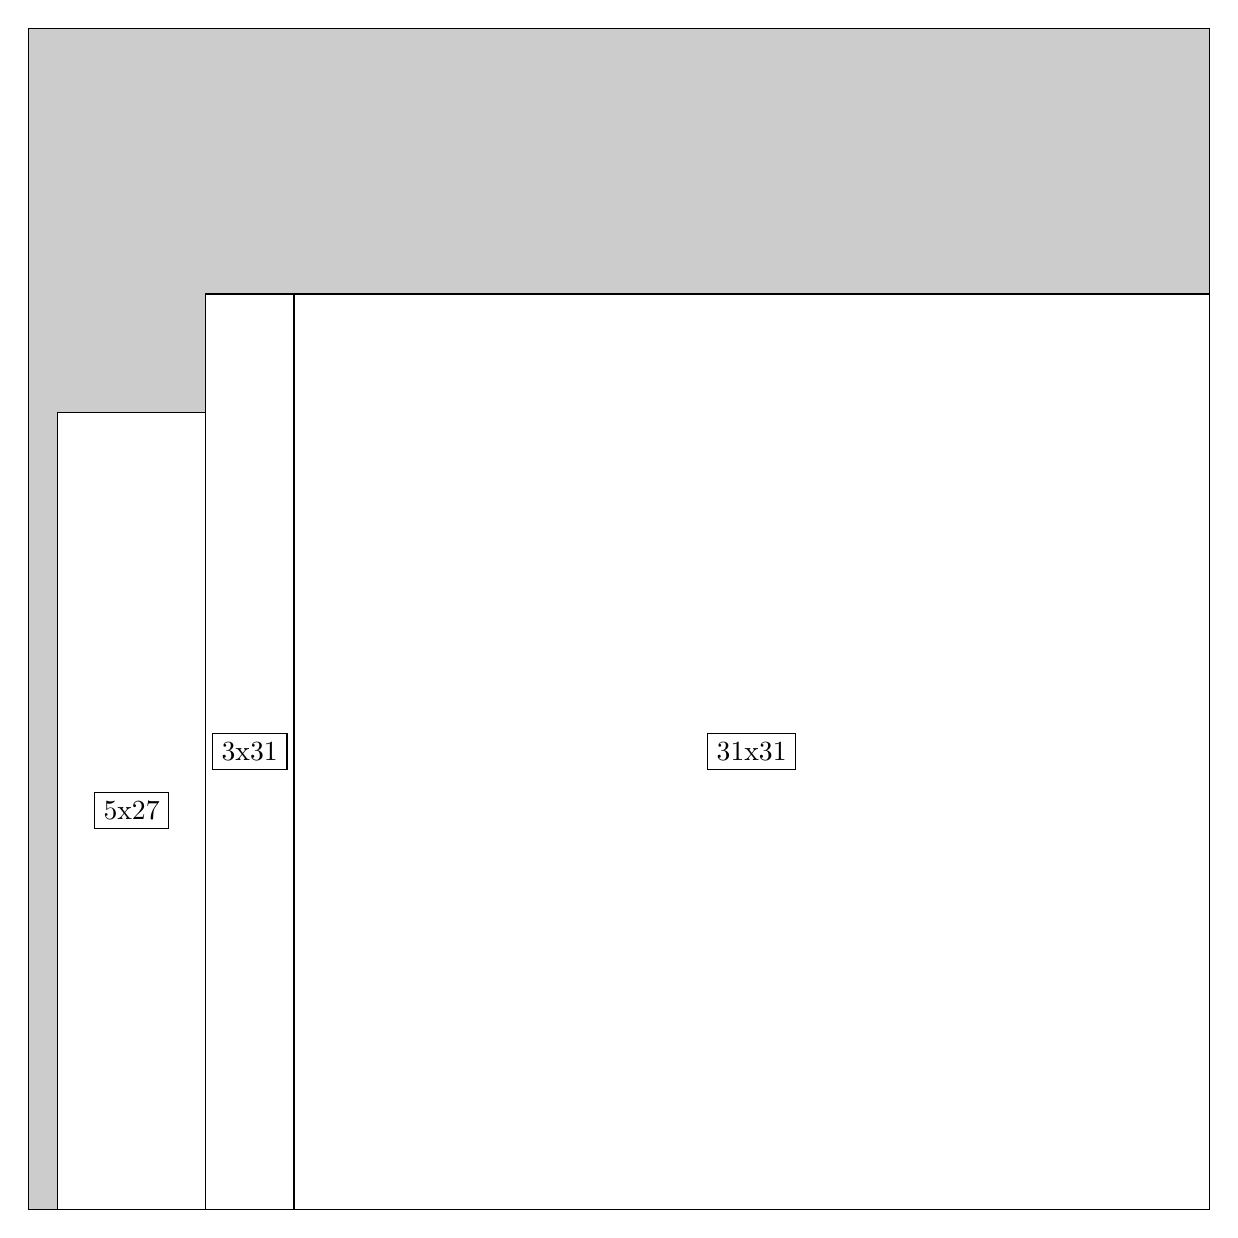
\begin{tikzpicture}[shorten >=1pt,scale=1.0,every node/.style={scale=1.0},->]
\tikzstyle{vertex}=[circle,fill=black!25,minimum size=14pt,inner sep=0pt]
\filldraw[fill=gray!40!white, draw=black] (0,0) rectangle (15.0,15.0);
\foreach \name/\x/\y/\w/\h in {31x31/3.375/0.0/11.625/11.625,3x31/2.25/0.0/1.125/11.625,5x27/0.375/0.0/1.875/10.125}
\filldraw[fill=white!40!white, draw=black] (\x,\y) rectangle node[draw] (\name) {\name} ++(\w,\h);
\end{tikzpicture}


w =31 , h =31 , x =9 , y =0 , v =961
\par
w =3 , h =31 , x =6 , y =0 , v =93
\par
w =5 , h =27 , x =1 , y =0 , v =135
\par
\newpage


\begin{tikzpicture}[shorten >=1pt,scale=1.0,every node/.style={scale=1.0},->]
\tikzstyle{vertex}=[circle,fill=black!25,minimum size=14pt,inner sep=0pt]
\filldraw[fill=gray!40!white, draw=black] (0,0) rectangle (15.0,15.0);
\foreach \name/\x/\y/\w/\h in {33x29/2.625/0.0/12.375/10.875,32x11/3.0/10.875/12.0/4.125,7x30/0.0/0.0/2.625/11.25,6x10/0.375/11.25/2.25/3.75}
\filldraw[fill=white!40!white, draw=black] (\x,\y) rectangle node[draw] (\name) {\name} ++(\w,\h);
\end{tikzpicture}


w =33 , h =29 , x =7 , y =0 , v =957
\par
w =32 , h =11 , x =8 , y =29 , v =352
\par
w =7 , h =30 , x =0 , y =0 , v =210
\par
w =6 , h =10 , x =1 , y =30 , v =60
\par
\newpage


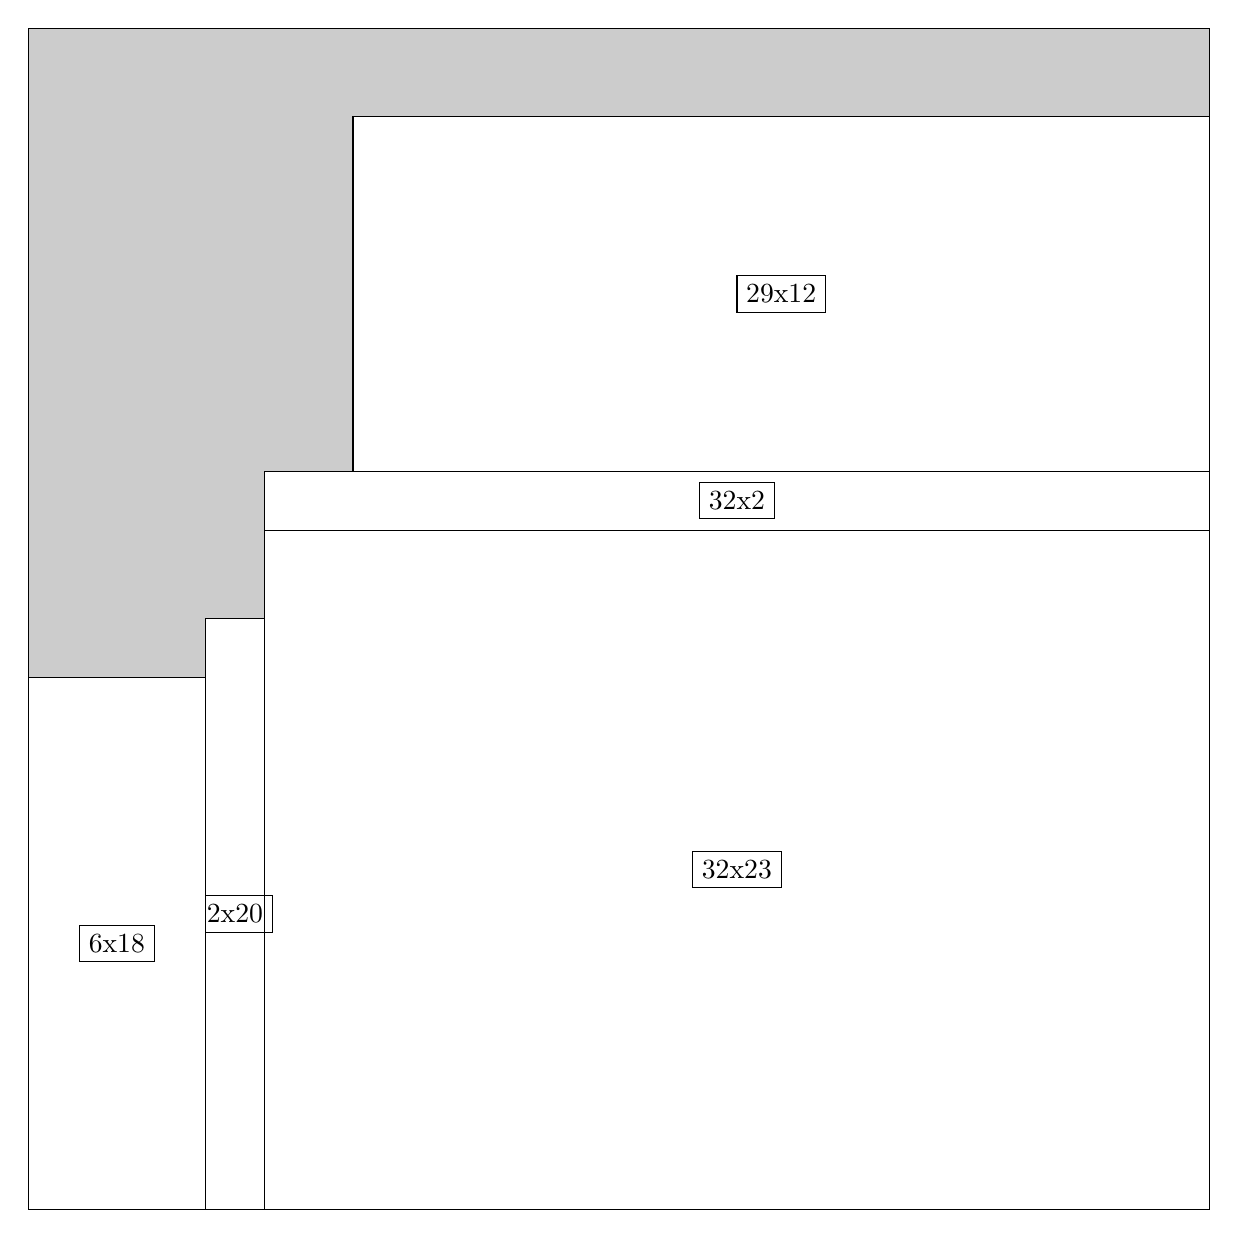
\begin{tikzpicture}[shorten >=1pt,scale=1.0,every node/.style={scale=1.0},->]
\tikzstyle{vertex}=[circle,fill=black!25,minimum size=14pt,inner sep=0pt]
\filldraw[fill=gray!40!white, draw=black] (0,0) rectangle (15.0,15.0);
\foreach \name/\x/\y/\w/\h in {32x23/3.0/0.0/12.0/8.625,2x20/2.25/0.0/0.75/7.5,6x18/0.0/0.0/2.25/6.75,32x2/3.0/8.625/12.0/0.75,29x12/4.125/9.375/10.875/4.5}
\filldraw[fill=white!40!white, draw=black] (\x,\y) rectangle node[draw] (\name) {\name} ++(\w,\h);
\end{tikzpicture}


w =32 , h =23 , x =8 , y =0 , v =736
\par
w =2 , h =20 , x =6 , y =0 , v =40
\par
w =6 , h =18 , x =0 , y =0 , v =108
\par
w =32 , h =2 , x =8 , y =23 , v =64
\par
w =29 , h =12 , x =11 , y =25 , v =348
\par
\newpage


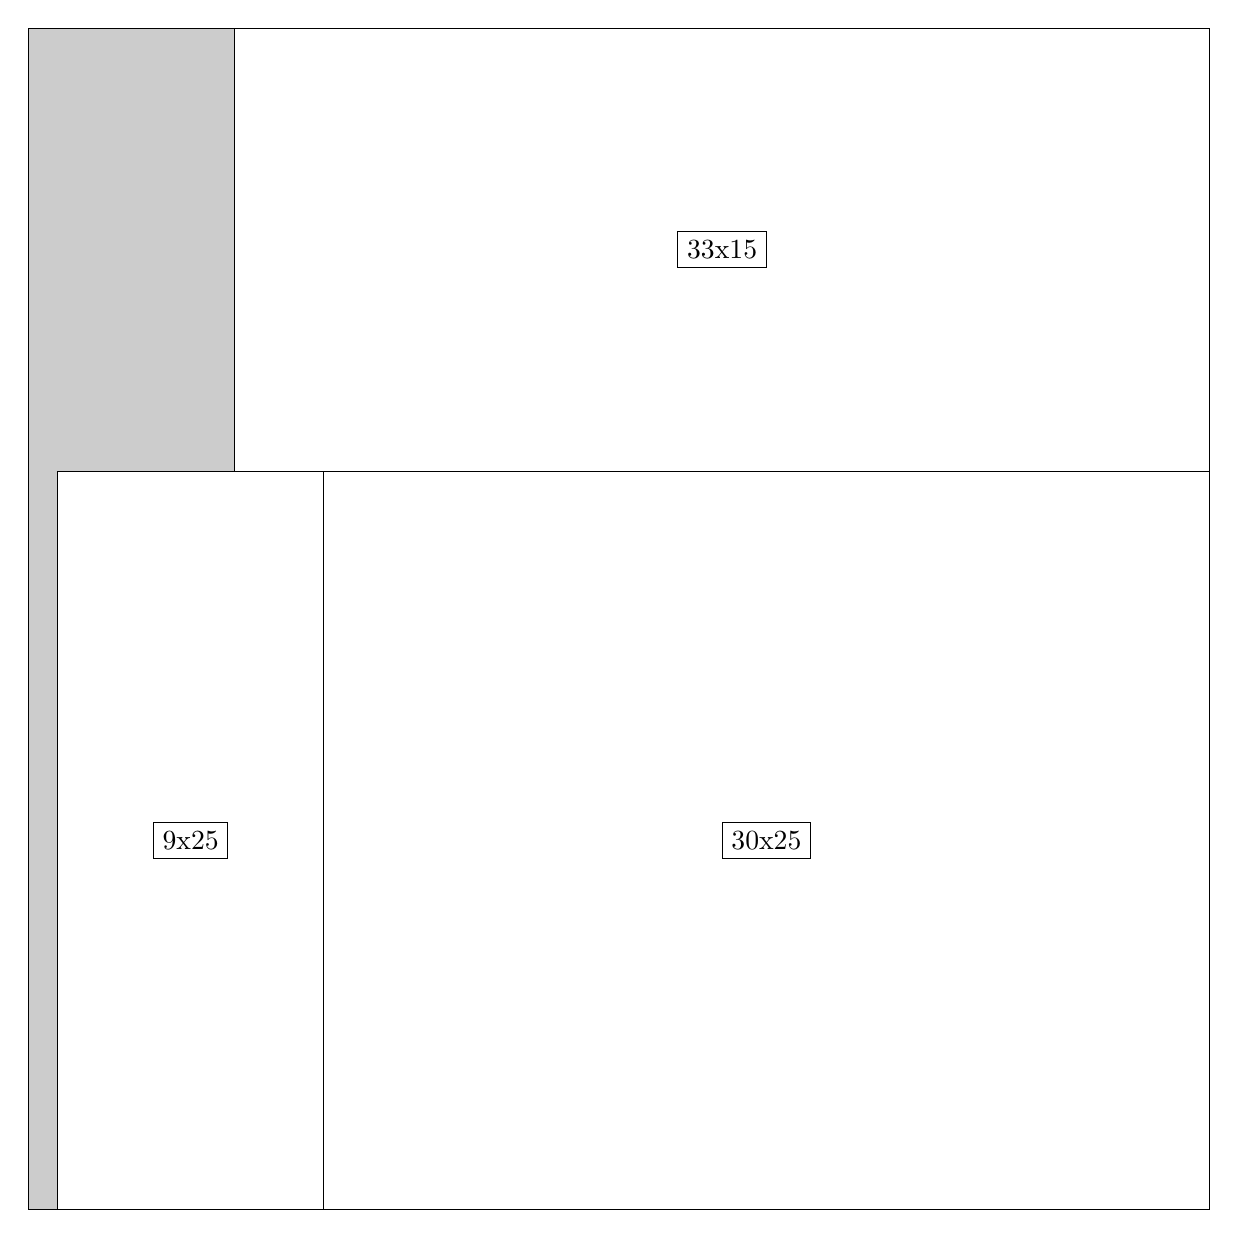
\begin{tikzpicture}[shorten >=1pt,scale=1.0,every node/.style={scale=1.0},->]
\tikzstyle{vertex}=[circle,fill=black!25,minimum size=14pt,inner sep=0pt]
\filldraw[fill=gray!40!white, draw=black] (0,0) rectangle (15.0,15.0);
\foreach \name/\x/\y/\w/\h in {30x25/3.75/0.0/11.25/9.375,9x25/0.375/0.0/3.375/9.375,33x15/2.625/9.375/12.375/5.625}
\filldraw[fill=white!40!white, draw=black] (\x,\y) rectangle node[draw] (\name) {\name} ++(\w,\h);
\end{tikzpicture}


w =30 , h =25 , x =10 , y =0 , v =750
\par
w =9 , h =25 , x =1 , y =0 , v =225
\par
w =33 , h =15 , x =7 , y =25 , v =495
\par
\newpage


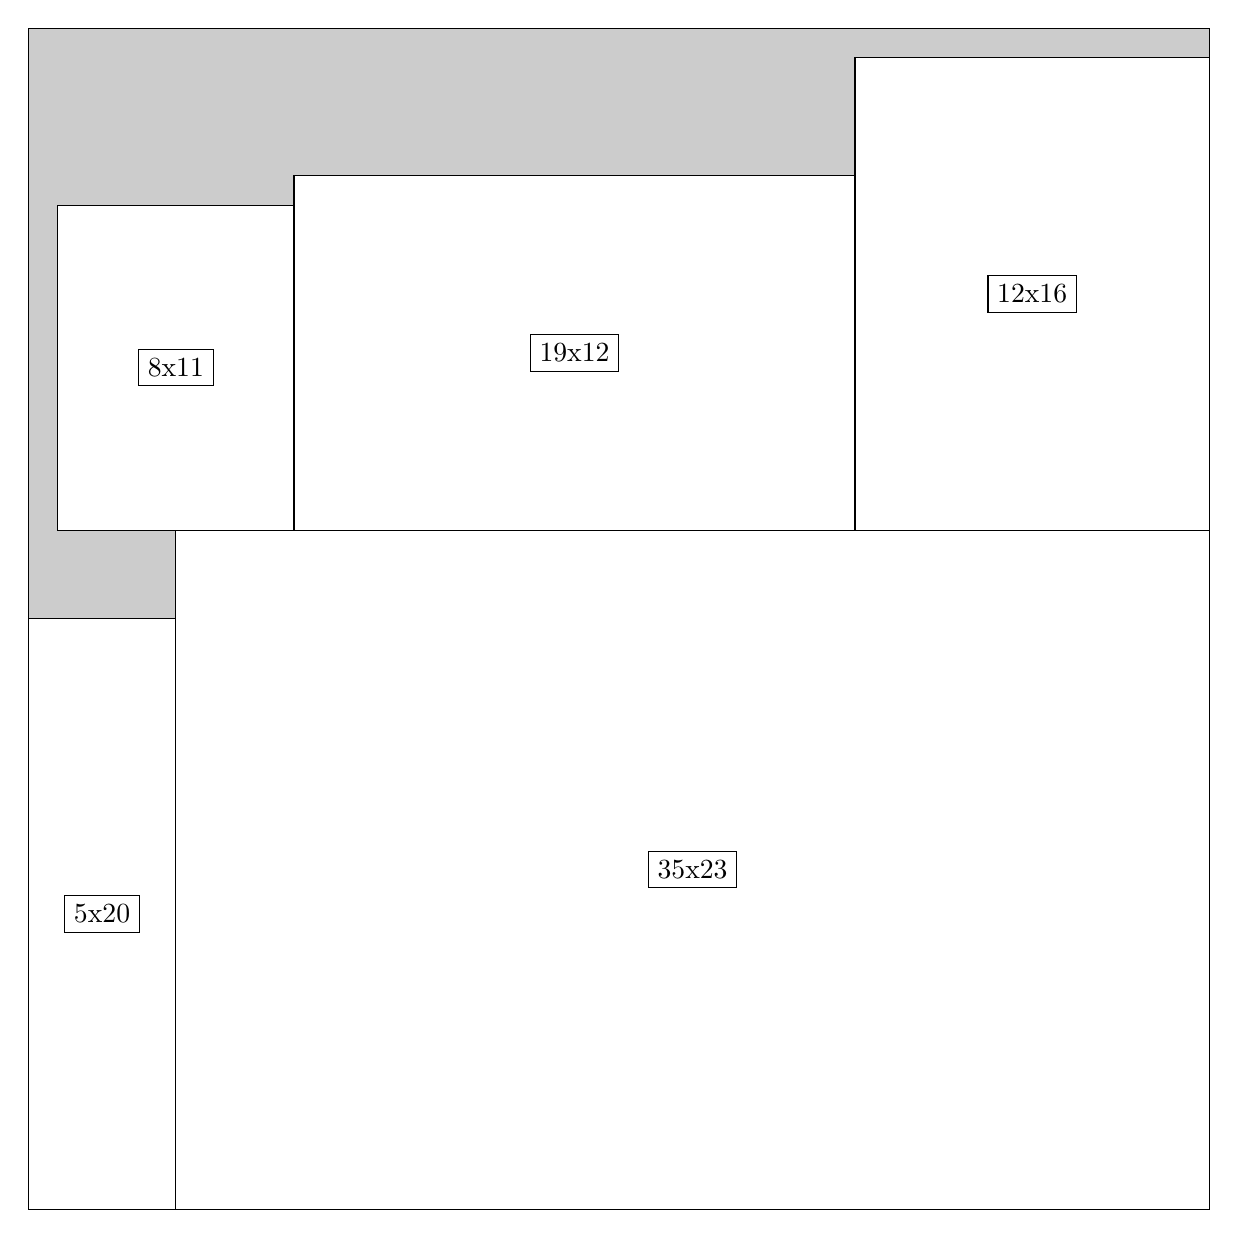
\begin{tikzpicture}[shorten >=1pt,scale=1.0,every node/.style={scale=1.0},->]
\tikzstyle{vertex}=[circle,fill=black!25,minimum size=14pt,inner sep=0pt]
\filldraw[fill=gray!40!white, draw=black] (0,0) rectangle (15.0,15.0);
\foreach \name/\x/\y/\w/\h in {35x23/1.875/0.0/13.125/8.625,5x20/0.0/0.0/1.875/7.5,12x16/10.5/8.625/4.5/6.0,19x12/3.375/8.625/7.125/4.5,8x11/0.375/8.625/3.0/4.125}
\filldraw[fill=white!40!white, draw=black] (\x,\y) rectangle node[draw] (\name) {\name} ++(\w,\h);
\end{tikzpicture}


w =35 , h =23 , x =5 , y =0 , v =805
\par
w =5 , h =20 , x =0 , y =0 , v =100
\par
w =12 , h =16 , x =28 , y =23 , v =192
\par
w =19 , h =12 , x =9 , y =23 , v =228
\par
w =8 , h =11 , x =1 , y =23 , v =88
\par
\newpage


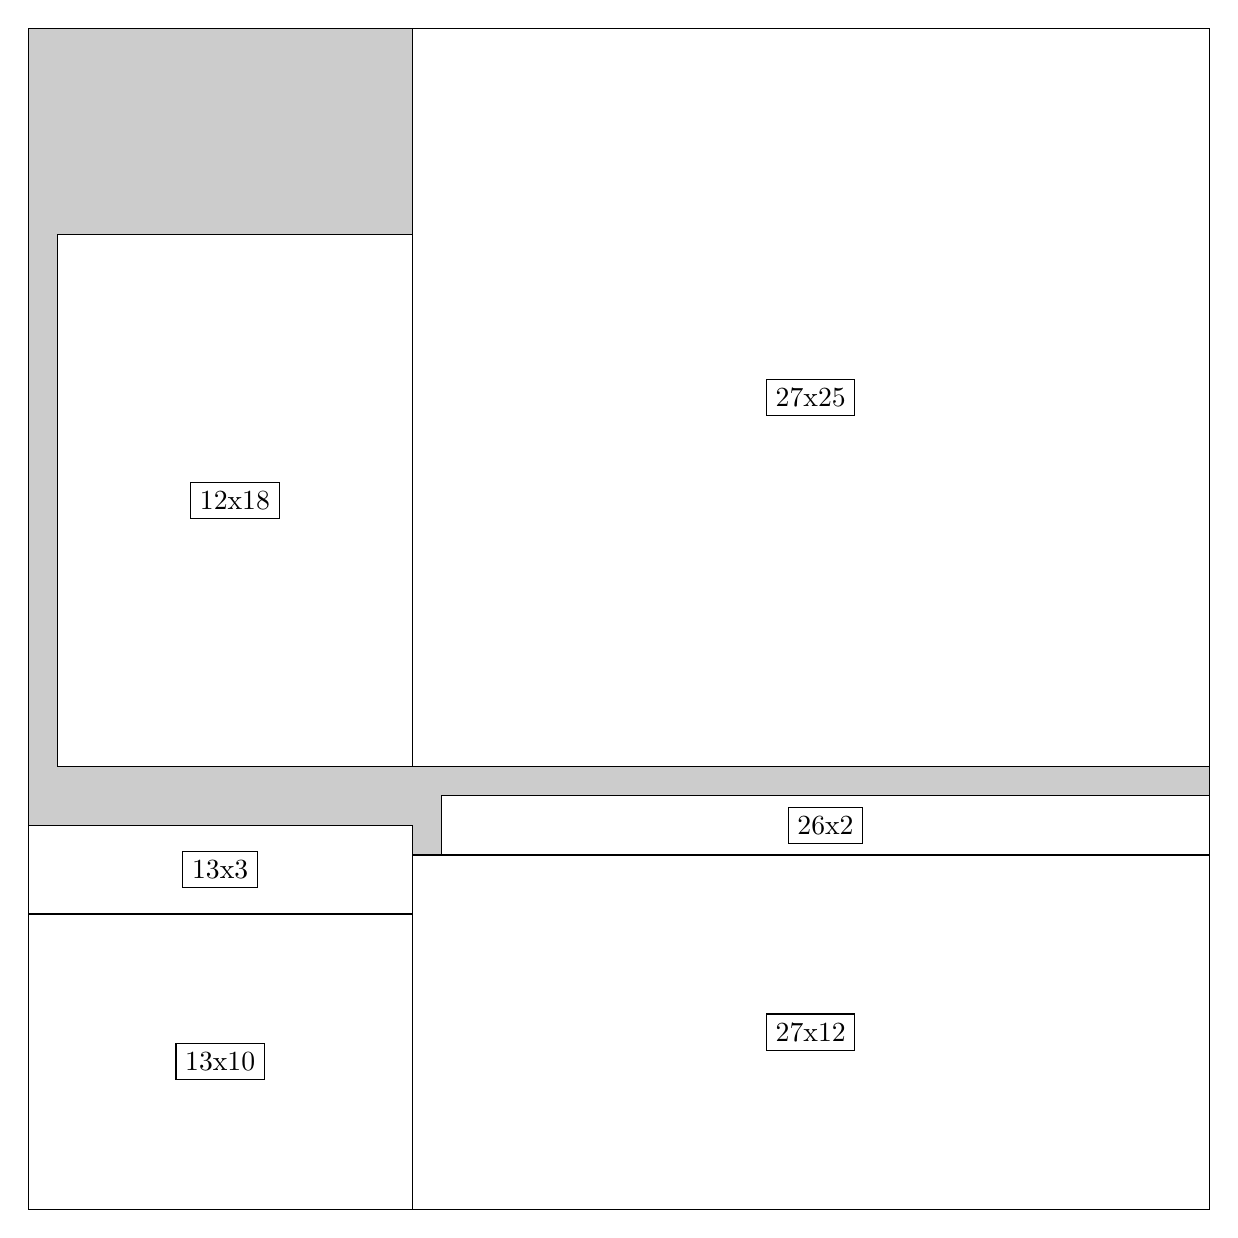
\begin{tikzpicture}[shorten >=1pt,scale=1.0,every node/.style={scale=1.0},->]
\tikzstyle{vertex}=[circle,fill=black!25,minimum size=14pt,inner sep=0pt]
\filldraw[fill=gray!40!white, draw=black] (0,0) rectangle (15.0,15.0);
\foreach \name/\x/\y/\w/\h in {27x12/4.875/0.0/10.125/4.5,26x2/5.25/4.5/9.75/0.75,13x10/0.0/0.0/4.875/3.75,13x3/0.0/3.75/4.875/1.125,27x25/4.875/5.625/10.125/9.375,12x18/0.375/5.625/4.5/6.75}
\filldraw[fill=white!40!white, draw=black] (\x,\y) rectangle node[draw] (\name) {\name} ++(\w,\h);
\end{tikzpicture}


w =27 , h =12 , x =13 , y =0 , v =324
\par
w =26 , h =2 , x =14 , y =12 , v =52
\par
w =13 , h =10 , x =0 , y =0 , v =130
\par
w =13 , h =3 , x =0 , y =10 , v =39
\par
w =27 , h =25 , x =13 , y =15 , v =675
\par
w =12 , h =18 , x =1 , y =15 , v =216
\par
\newpage


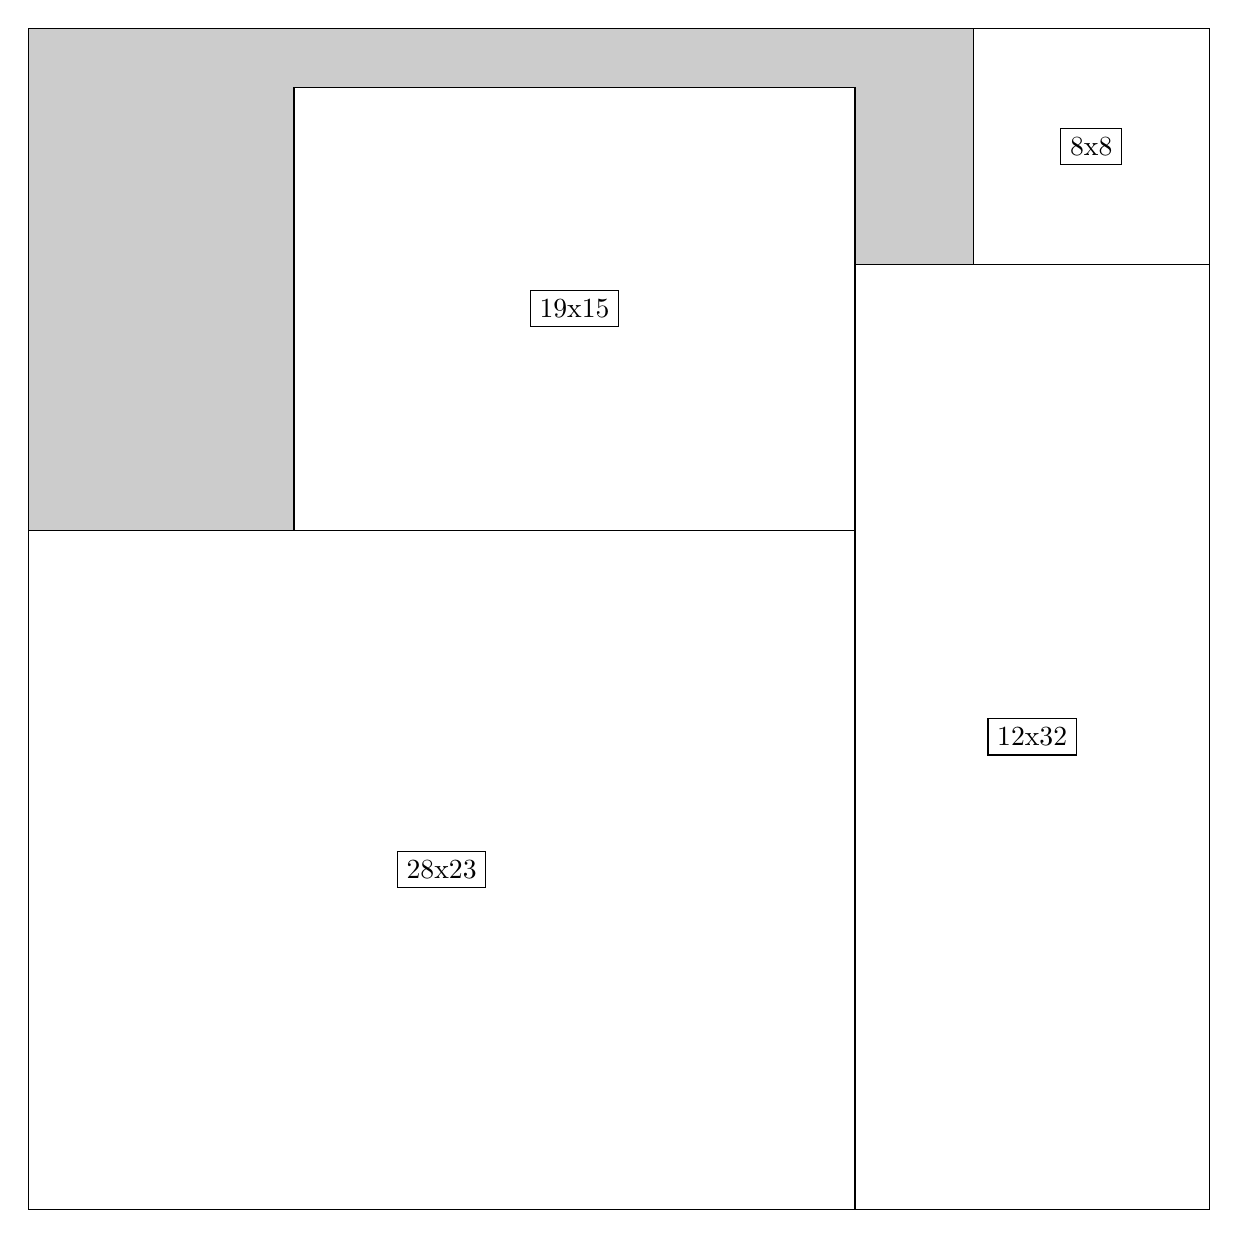
\begin{tikzpicture}[shorten >=1pt,scale=1.0,every node/.style={scale=1.0},->]
\tikzstyle{vertex}=[circle,fill=black!25,minimum size=14pt,inner sep=0pt]
\filldraw[fill=gray!40!white, draw=black] (0,0) rectangle (15.0,15.0);
\foreach \name/\x/\y/\w/\h in {12x32/10.5/0.0/4.5/12.0,8x8/12.0/12.0/3.0/3.0,28x23/0.0/0.0/10.5/8.625,19x15/3.375/8.625/7.125/5.625}
\filldraw[fill=white!40!white, draw=black] (\x,\y) rectangle node[draw] (\name) {\name} ++(\w,\h);
\end{tikzpicture}


w =12 , h =32 , x =28 , y =0 , v =384
\par
w =8 , h =8 , x =32 , y =32 , v =64
\par
w =28 , h =23 , x =0 , y =0 , v =644
\par
w =19 , h =15 , x =9 , y =23 , v =285
\par
\newpage


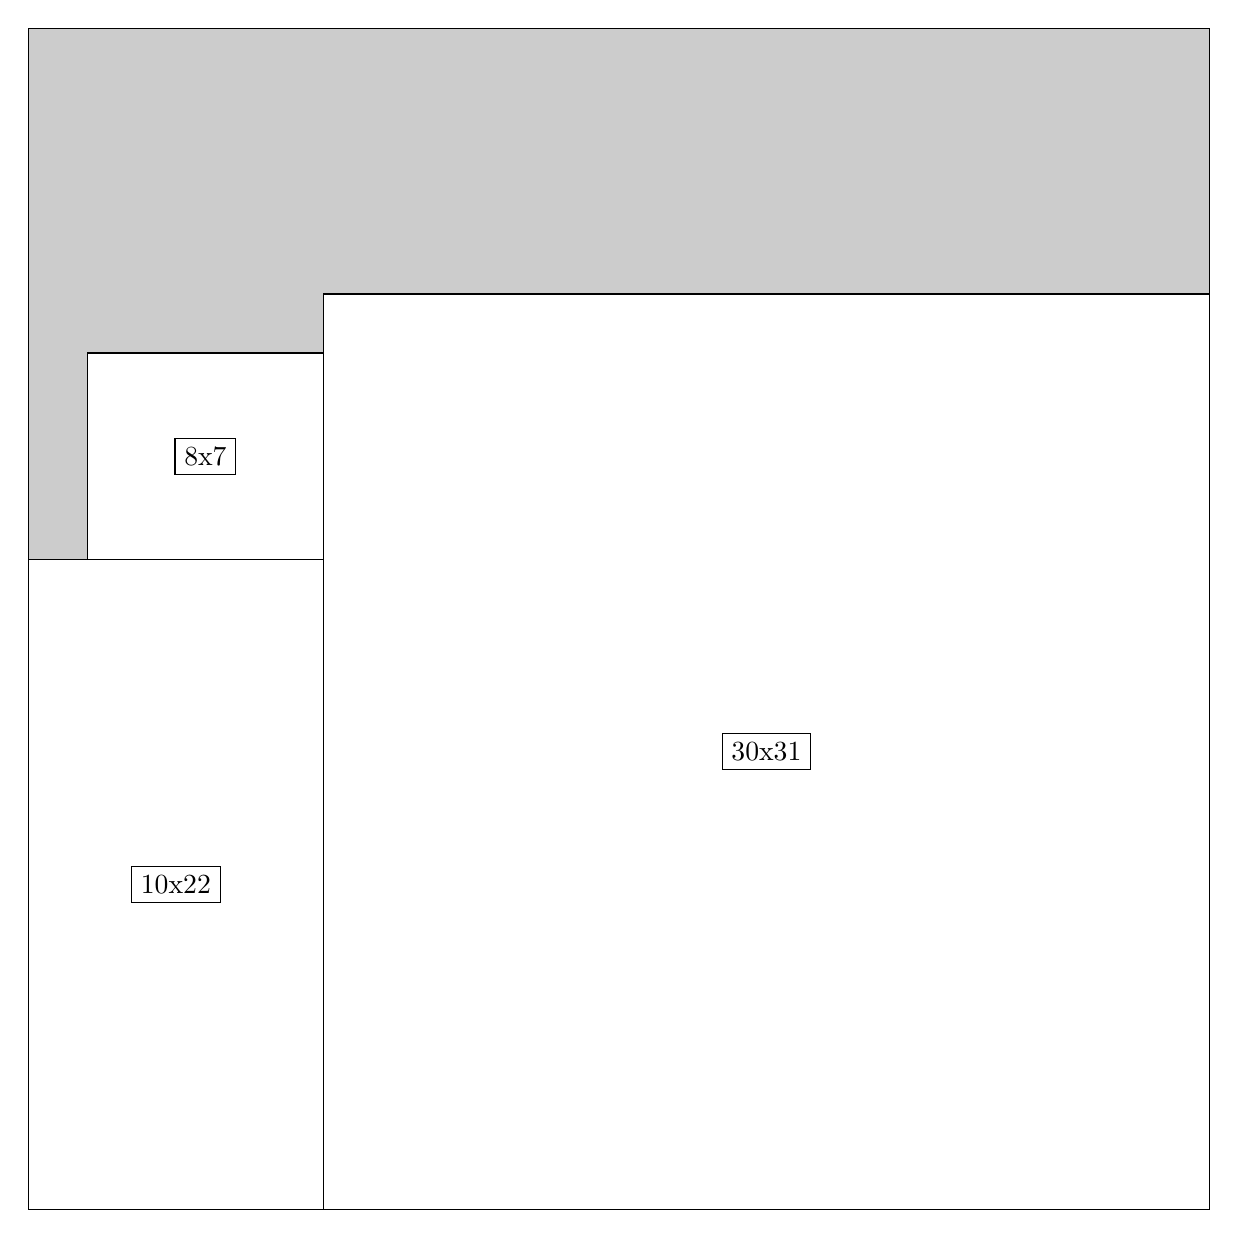
\begin{tikzpicture}[shorten >=1pt,scale=1.0,every node/.style={scale=1.0},->]
\tikzstyle{vertex}=[circle,fill=black!25,minimum size=14pt,inner sep=0pt]
\filldraw[fill=gray!40!white, draw=black] (0,0) rectangle (15.0,15.0);
\foreach \name/\x/\y/\w/\h in {30x31/3.75/0.0/11.25/11.625,10x22/0.0/0.0/3.75/8.25,8x7/0.75/8.25/3.0/2.625}
\filldraw[fill=white!40!white, draw=black] (\x,\y) rectangle node[draw] (\name) {\name} ++(\w,\h);
\end{tikzpicture}


w =30 , h =31 , x =10 , y =0 , v =930
\par
w =10 , h =22 , x =0 , y =0 , v =220
\par
w =8 , h =7 , x =2 , y =22 , v =56
\par
\newpage


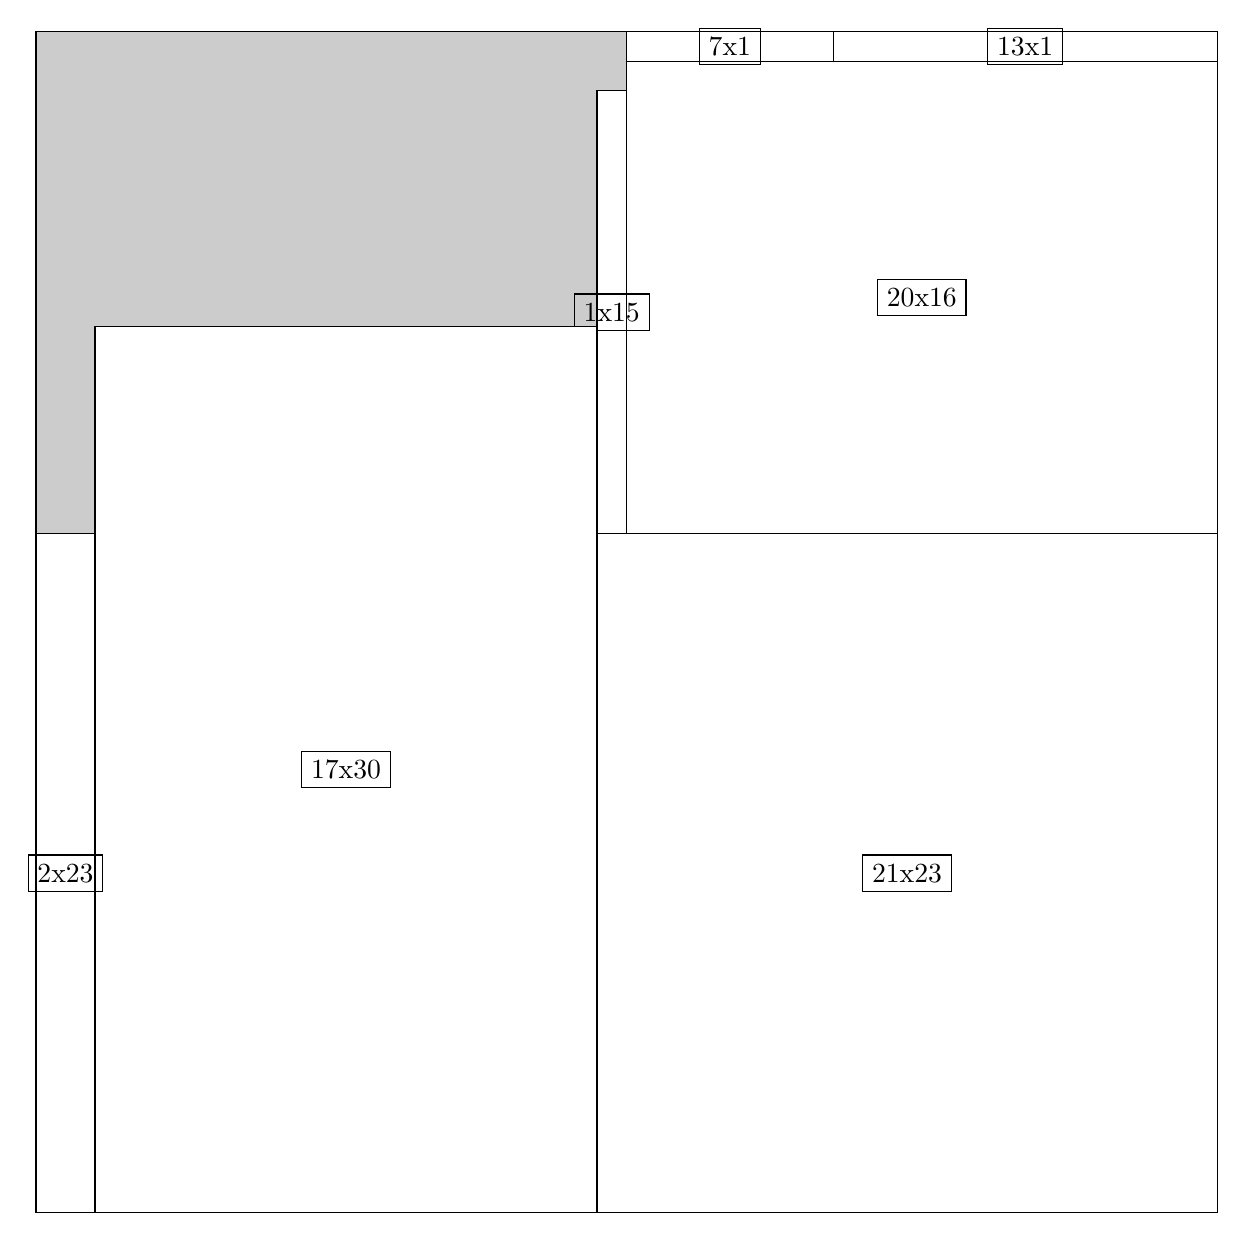
\begin{tikzpicture}[shorten >=1pt,scale=1.0,every node/.style={scale=1.0},->]
\tikzstyle{vertex}=[circle,fill=black!25,minimum size=14pt,inner sep=0pt]
\filldraw[fill=gray!40!white, draw=black] (0,0) rectangle (15.0,15.0);
\foreach \name/\x/\y/\w/\h in {21x23/7.125/0.0/7.875/8.625,20x16/7.5/8.625/7.5/6.0,1x15/7.125/8.625/0.375/5.625,13x1/10.125/14.625/4.875/0.375,7x1/7.5/14.625/2.625/0.375,17x30/0.75/0.0/6.375/11.25,2x23/0.0/0.0/0.75/8.625}
\filldraw[fill=white!40!white, draw=black] (\x,\y) rectangle node[draw] (\name) {\name} ++(\w,\h);
\end{tikzpicture}


w =21 , h =23 , x =19 , y =0 , v =483
\par
w =20 , h =16 , x =20 , y =23 , v =320
\par
w =1 , h =15 , x =19 , y =23 , v =15
\par
w =13 , h =1 , x =27 , y =39 , v =13
\par
w =7 , h =1 , x =20 , y =39 , v =7
\par
w =17 , h =30 , x =2 , y =0 , v =510
\par
w =2 , h =23 , x =0 , y =0 , v =46
\par
\newpage


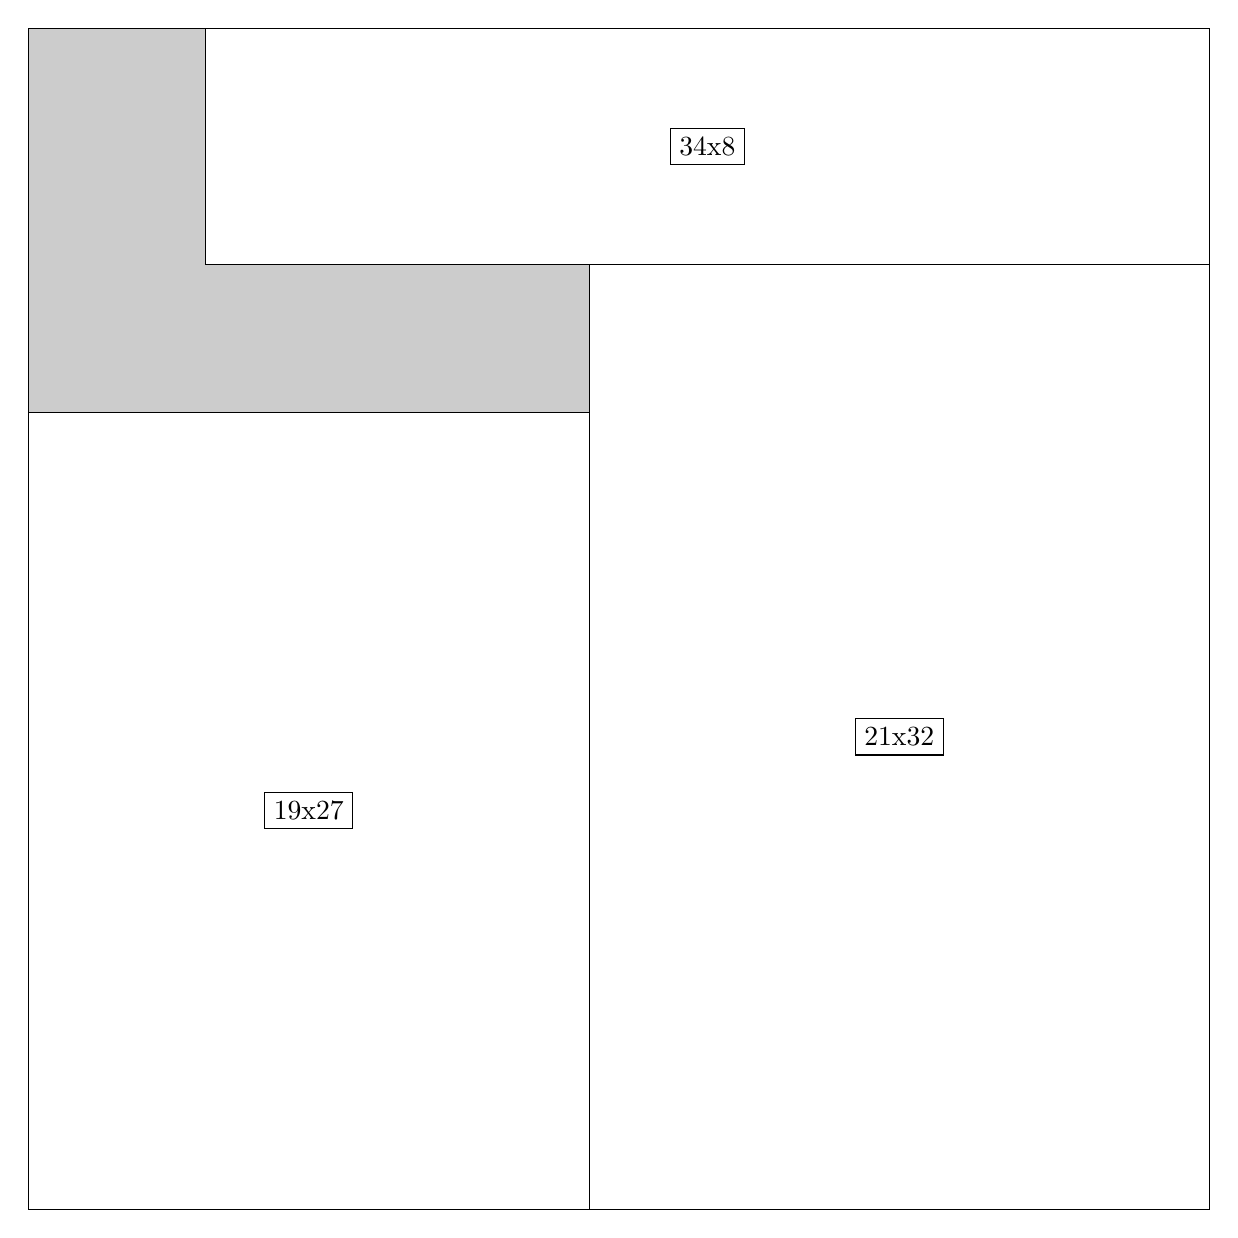
\begin{tikzpicture}[shorten >=1pt,scale=1.0,every node/.style={scale=1.0},->]
\tikzstyle{vertex}=[circle,fill=black!25,minimum size=14pt,inner sep=0pt]
\filldraw[fill=gray!40!white, draw=black] (0,0) rectangle (15.0,15.0);
\foreach \name/\x/\y/\w/\h in {21x32/7.125/0.0/7.875/12.0,19x27/0.0/0.0/7.125/10.125,34x8/2.25/12.0/12.75/3.0}
\filldraw[fill=white!40!white, draw=black] (\x,\y) rectangle node[draw] (\name) {\name} ++(\w,\h);
\end{tikzpicture}


w =21 , h =32 , x =19 , y =0 , v =672
\par
w =19 , h =27 , x =0 , y =0 , v =513
\par
w =34 , h =8 , x =6 , y =32 , v =272
\par
\newpage


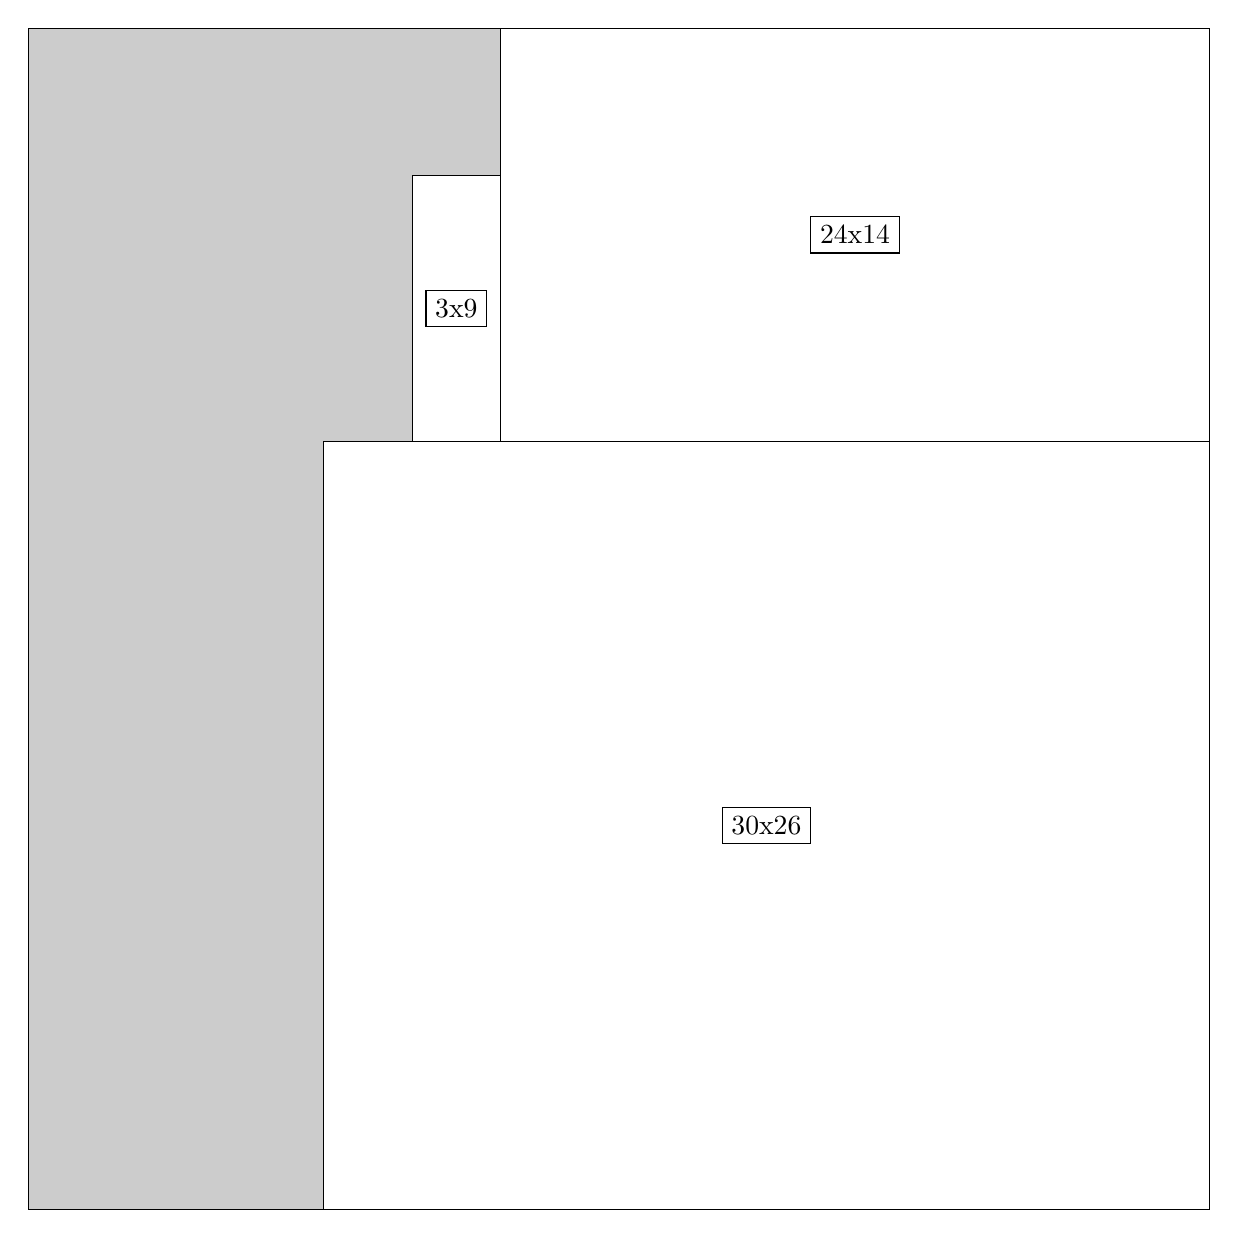
\begin{tikzpicture}[shorten >=1pt,scale=1.0,every node/.style={scale=1.0},->]
\tikzstyle{vertex}=[circle,fill=black!25,minimum size=14pt,inner sep=0pt]
\filldraw[fill=gray!40!white, draw=black] (0,0) rectangle (15.0,15.0);
\foreach \name/\x/\y/\w/\h in {30x26/3.75/0.0/11.25/9.75,24x14/6.0/9.75/9.0/5.25,3x9/4.875/9.75/1.125/3.375}
\filldraw[fill=white!40!white, draw=black] (\x,\y) rectangle node[draw] (\name) {\name} ++(\w,\h);
\end{tikzpicture}


w =30 , h =26 , x =10 , y =0 , v =780
\par
w =24 , h =14 , x =16 , y =26 , v =336
\par
w =3 , h =9 , x =13 , y =26 , v =27
\par
\newpage


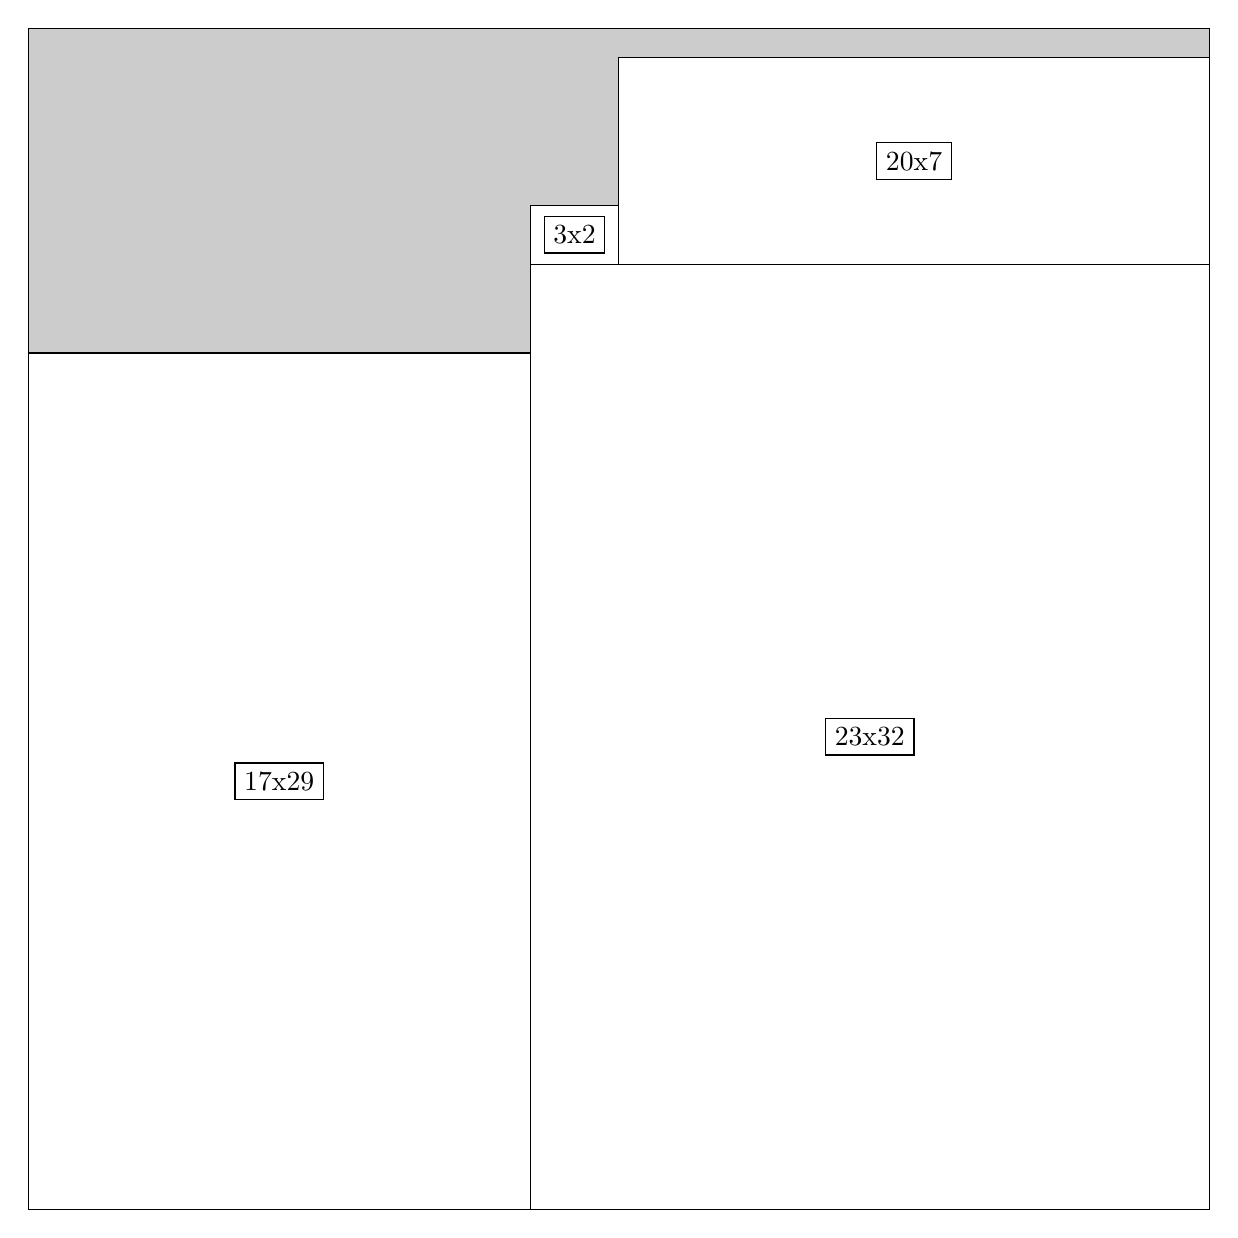
\begin{tikzpicture}[shorten >=1pt,scale=1.0,every node/.style={scale=1.0},->]
\tikzstyle{vertex}=[circle,fill=black!25,minimum size=14pt,inner sep=0pt]
\filldraw[fill=gray!40!white, draw=black] (0,0) rectangle (15.0,15.0);
\foreach \name/\x/\y/\w/\h in {23x32/6.375/0.0/8.625/12.0,20x7/7.5/12.0/7.5/2.625,3x2/6.375/12.0/1.125/0.75,17x29/0.0/0.0/6.375/10.875}
\filldraw[fill=white!40!white, draw=black] (\x,\y) rectangle node[draw] (\name) {\name} ++(\w,\h);
\end{tikzpicture}


w =23 , h =32 , x =17 , y =0 , v =736
\par
w =20 , h =7 , x =20 , y =32 , v =140
\par
w =3 , h =2 , x =17 , y =32 , v =6
\par
w =17 , h =29 , x =0 , y =0 , v =493
\par
\newpage


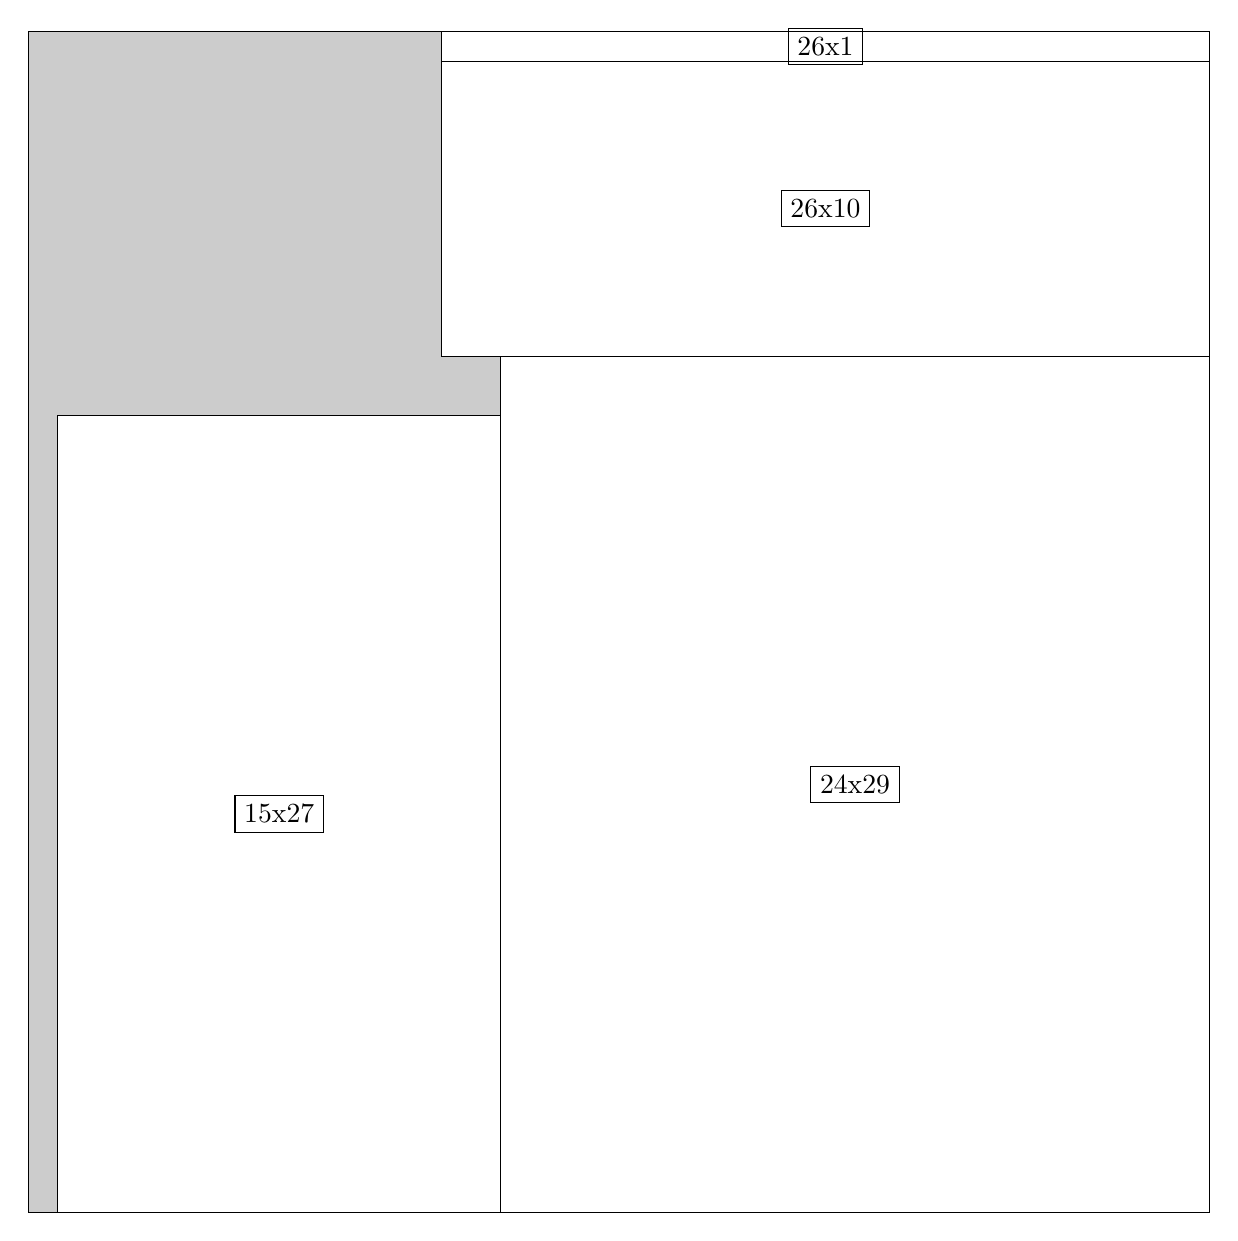
\begin{tikzpicture}[shorten >=1pt,scale=1.0,every node/.style={scale=1.0},->]
\tikzstyle{vertex}=[circle,fill=black!25,minimum size=14pt,inner sep=0pt]
\filldraw[fill=gray!40!white, draw=black] (0,0) rectangle (15.0,15.0);
\foreach \name/\x/\y/\w/\h in {24x29/6.0/0.0/9.0/10.875,15x27/0.375/0.0/5.625/10.125,26x10/5.25/10.875/9.75/3.75,26x1/5.25/14.625/9.75/0.375}
\filldraw[fill=white!40!white, draw=black] (\x,\y) rectangle node[draw] (\name) {\name} ++(\w,\h);
\end{tikzpicture}


w =24 , h =29 , x =16 , y =0 , v =696
\par
w =15 , h =27 , x =1 , y =0 , v =405
\par
w =26 , h =10 , x =14 , y =29 , v =260
\par
w =26 , h =1 , x =14 , y =39 , v =26
\par
\newpage


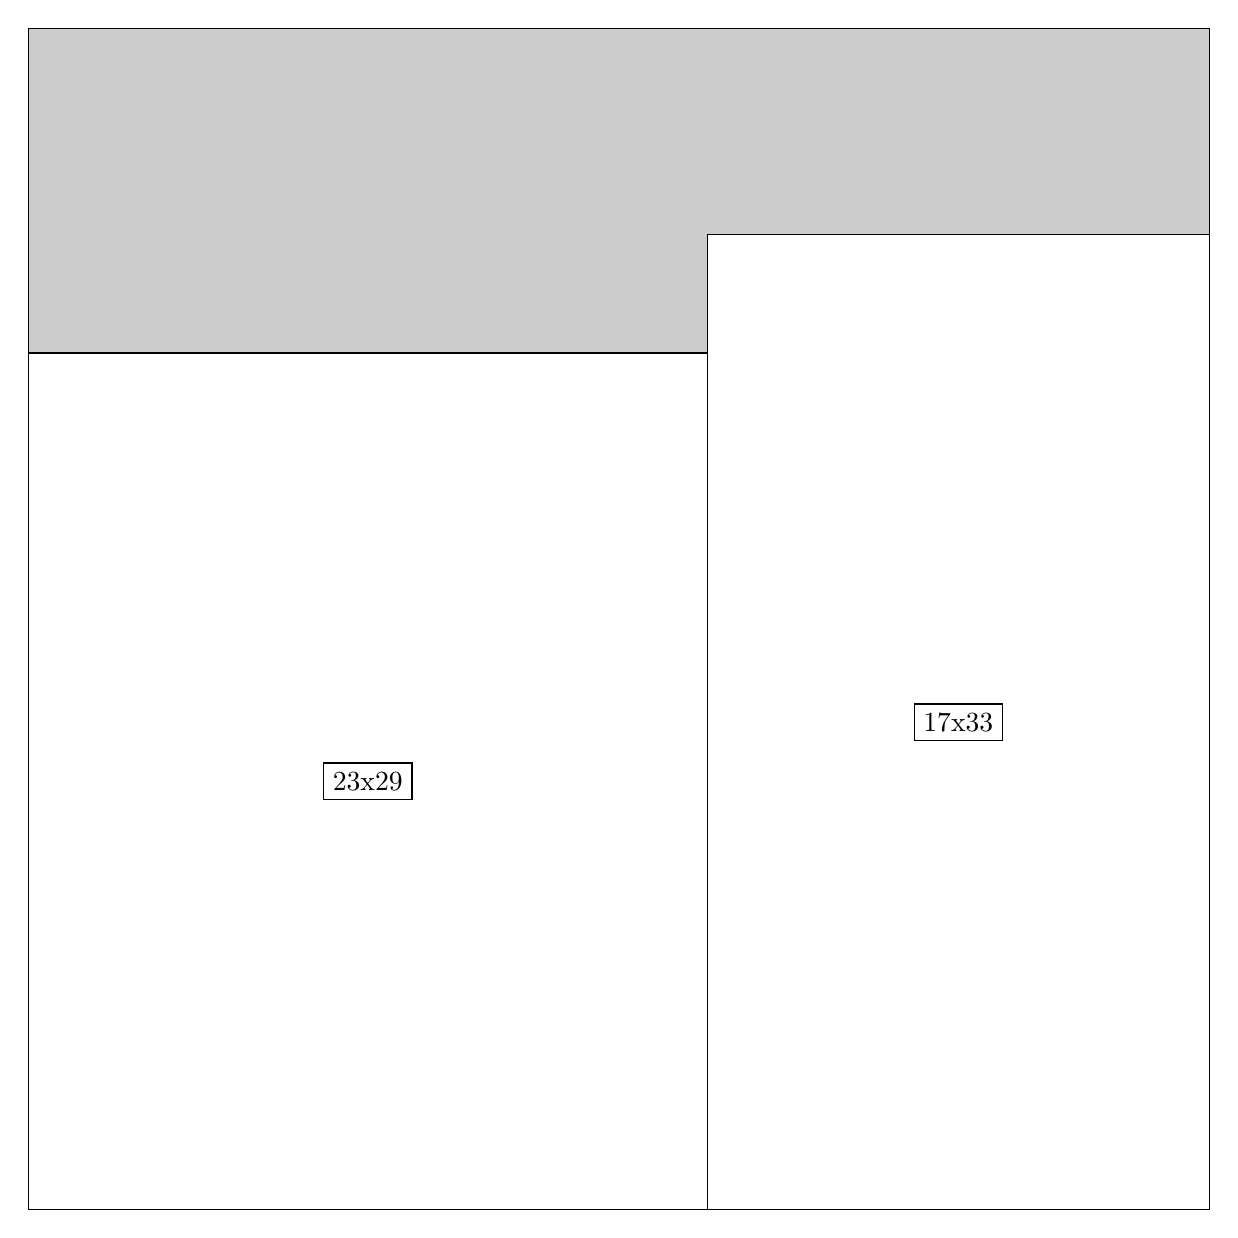
\begin{tikzpicture}[shorten >=1pt,scale=1.0,every node/.style={scale=1.0},->]
\tikzstyle{vertex}=[circle,fill=black!25,minimum size=14pt,inner sep=0pt]
\filldraw[fill=gray!40!white, draw=black] (0,0) rectangle (15.0,15.0);
\foreach \name/\x/\y/\w/\h in {17x33/8.625/0.0/6.375/12.375,23x29/0.0/0.0/8.625/10.875}
\filldraw[fill=white!40!white, draw=black] (\x,\y) rectangle node[draw] (\name) {\name} ++(\w,\h);
\end{tikzpicture}


w =17 , h =33 , x =23 , y =0 , v =561
\par
w =23 , h =29 , x =0 , y =0 , v =667
\par
\newpage


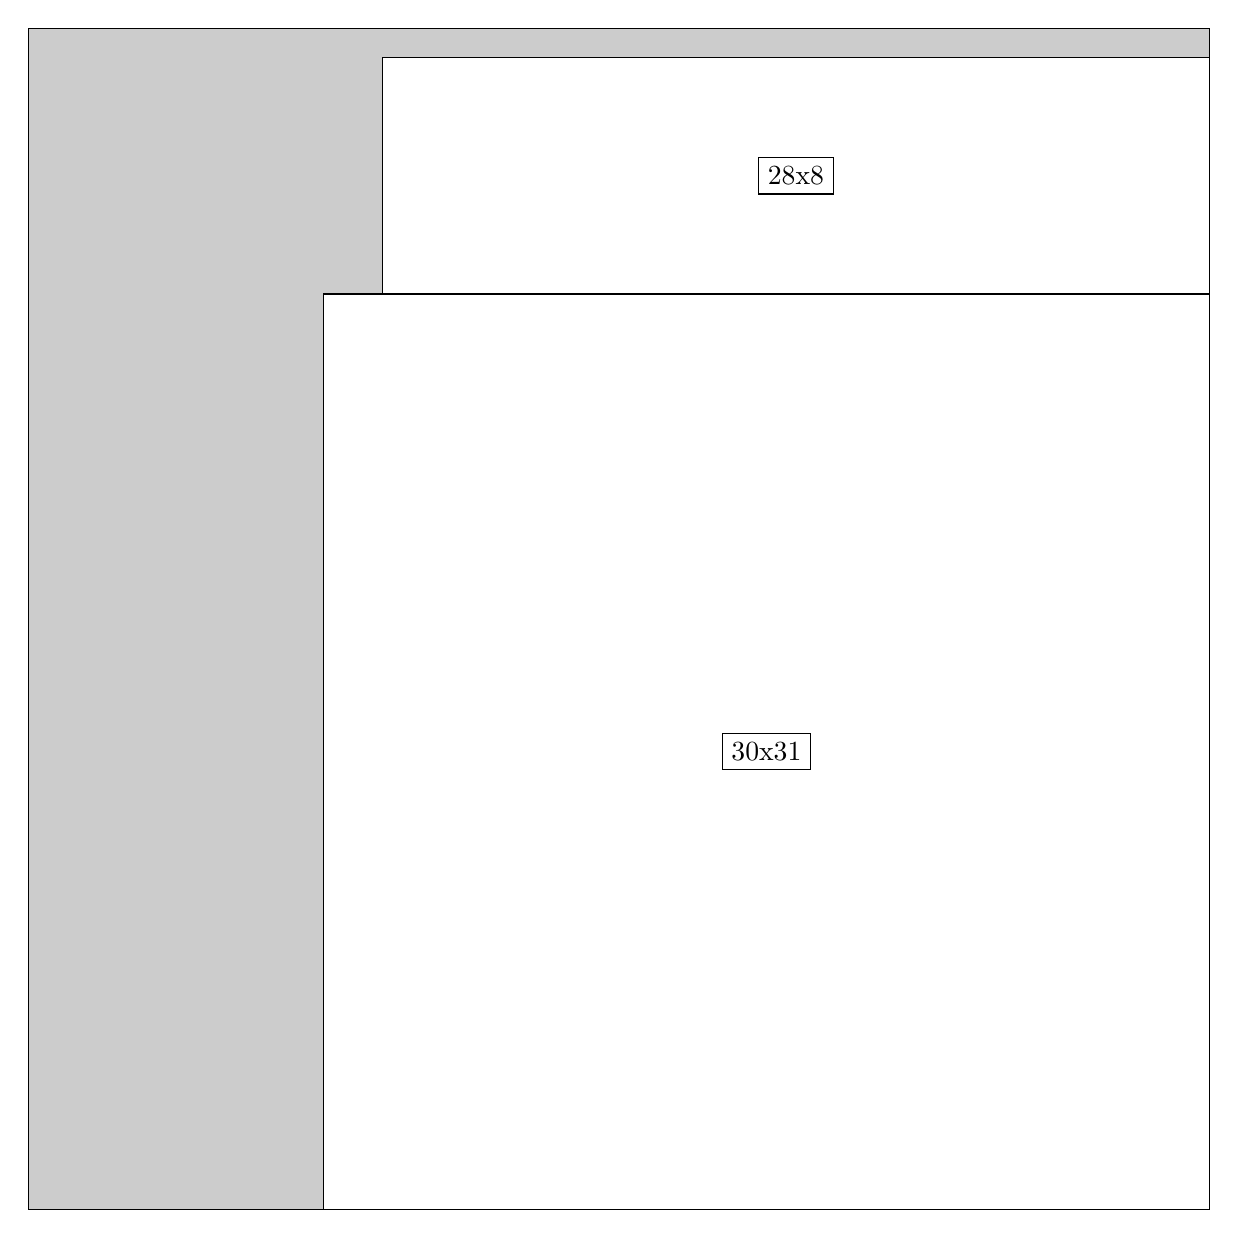
\begin{tikzpicture}[shorten >=1pt,scale=1.0,every node/.style={scale=1.0},->]
\tikzstyle{vertex}=[circle,fill=black!25,minimum size=14pt,inner sep=0pt]
\filldraw[fill=gray!40!white, draw=black] (0,0) rectangle (15.0,15.0);
\foreach \name/\x/\y/\w/\h in {30x31/3.75/0.0/11.25/11.625,28x8/4.5/11.625/10.5/3.0}
\filldraw[fill=white!40!white, draw=black] (\x,\y) rectangle node[draw] (\name) {\name} ++(\w,\h);
\end{tikzpicture}


w =30 , h =31 , x =10 , y =0 , v =930
\par
w =28 , h =8 , x =12 , y =31 , v =224
\par
\newpage


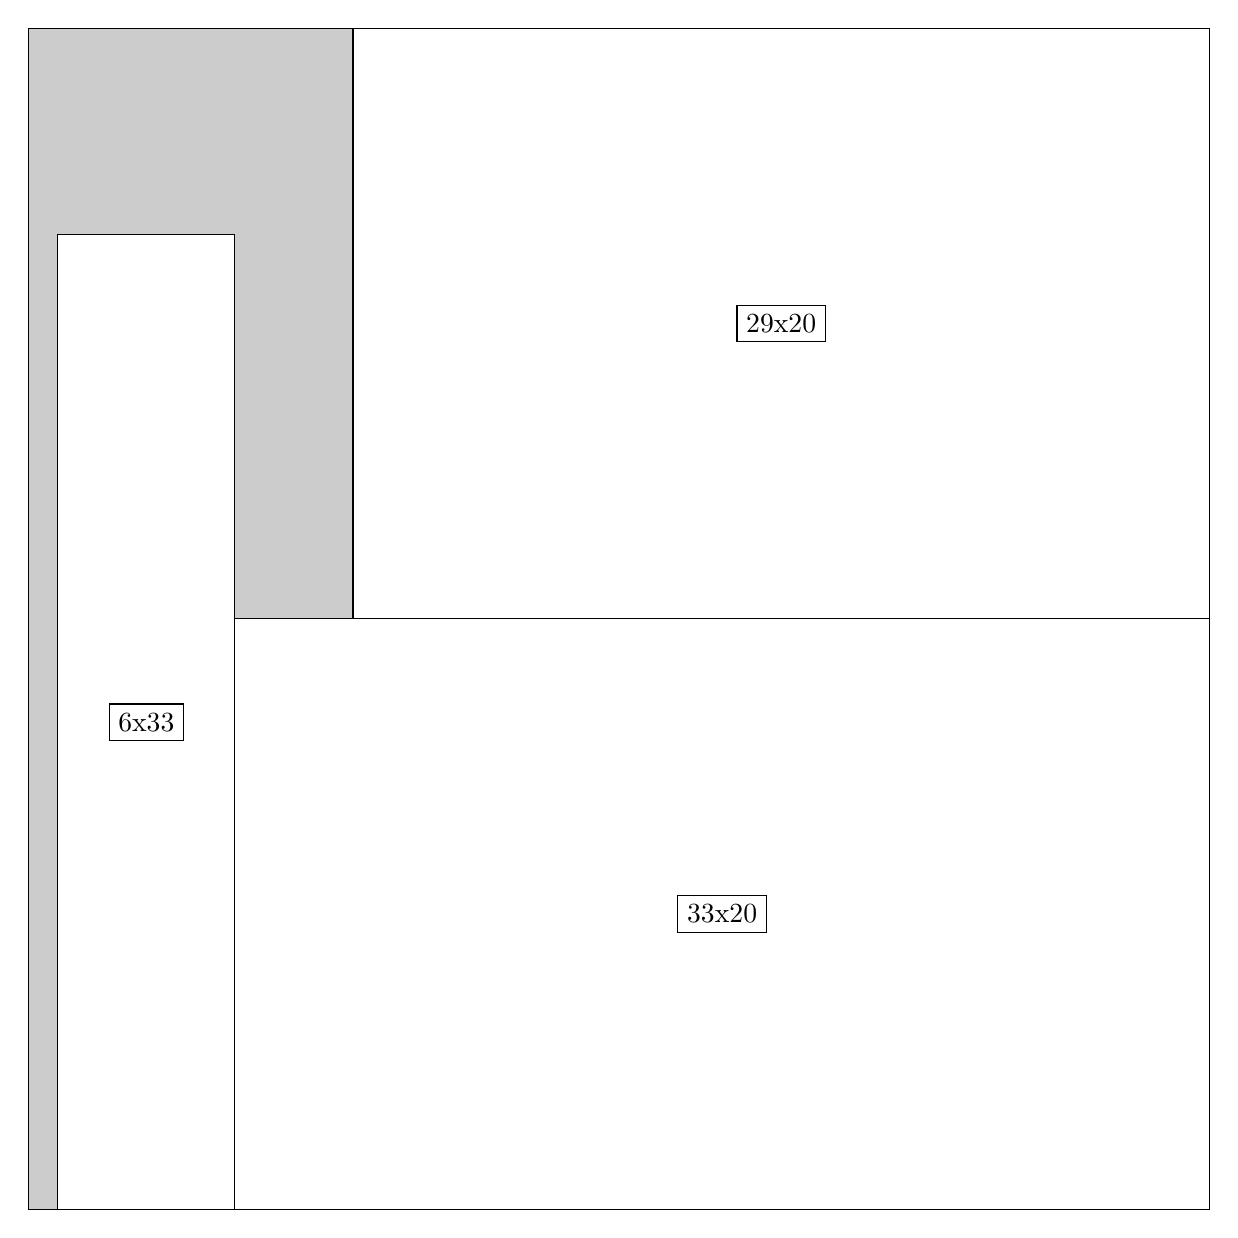
\begin{tikzpicture}[shorten >=1pt,scale=1.0,every node/.style={scale=1.0},->]
\tikzstyle{vertex}=[circle,fill=black!25,minimum size=14pt,inner sep=0pt]
\filldraw[fill=gray!40!white, draw=black] (0,0) rectangle (15.0,15.0);
\foreach \name/\x/\y/\w/\h in {33x20/2.625/0.0/12.375/7.5,29x20/4.125/7.5/10.875/7.5,6x33/0.375/0.0/2.25/12.375}
\filldraw[fill=white!40!white, draw=black] (\x,\y) rectangle node[draw] (\name) {\name} ++(\w,\h);
\end{tikzpicture}


w =33 , h =20 , x =7 , y =0 , v =660
\par
w =29 , h =20 , x =11 , y =20 , v =580
\par
w =6 , h =33 , x =1 , y =0 , v =198
\par
\newpage


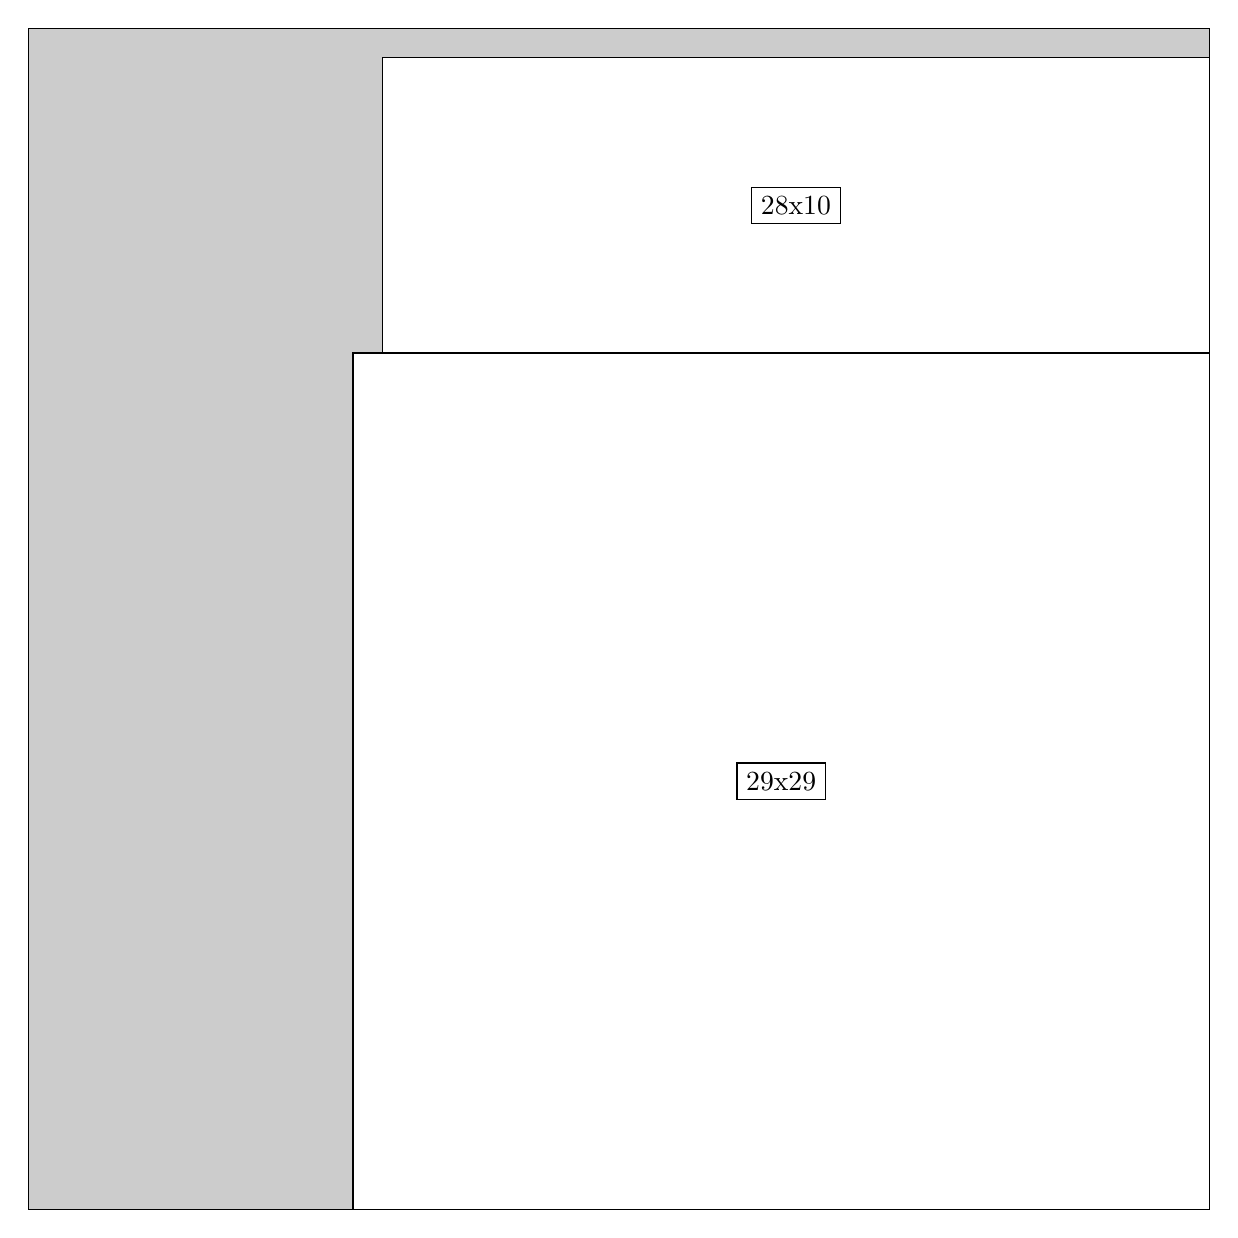
\begin{tikzpicture}[shorten >=1pt,scale=1.0,every node/.style={scale=1.0},->]
\tikzstyle{vertex}=[circle,fill=black!25,minimum size=14pt,inner sep=0pt]
\filldraw[fill=gray!40!white, draw=black] (0,0) rectangle (15.0,15.0);
\foreach \name/\x/\y/\w/\h in {29x29/4.125/0.0/10.875/10.875,28x10/4.5/10.875/10.5/3.75}
\filldraw[fill=white!40!white, draw=black] (\x,\y) rectangle node[draw] (\name) {\name} ++(\w,\h);
\end{tikzpicture}


w =29 , h =29 , x =11 , y =0 , v =841
\par
w =28 , h =10 , x =12 , y =29 , v =280
\par
\newpage


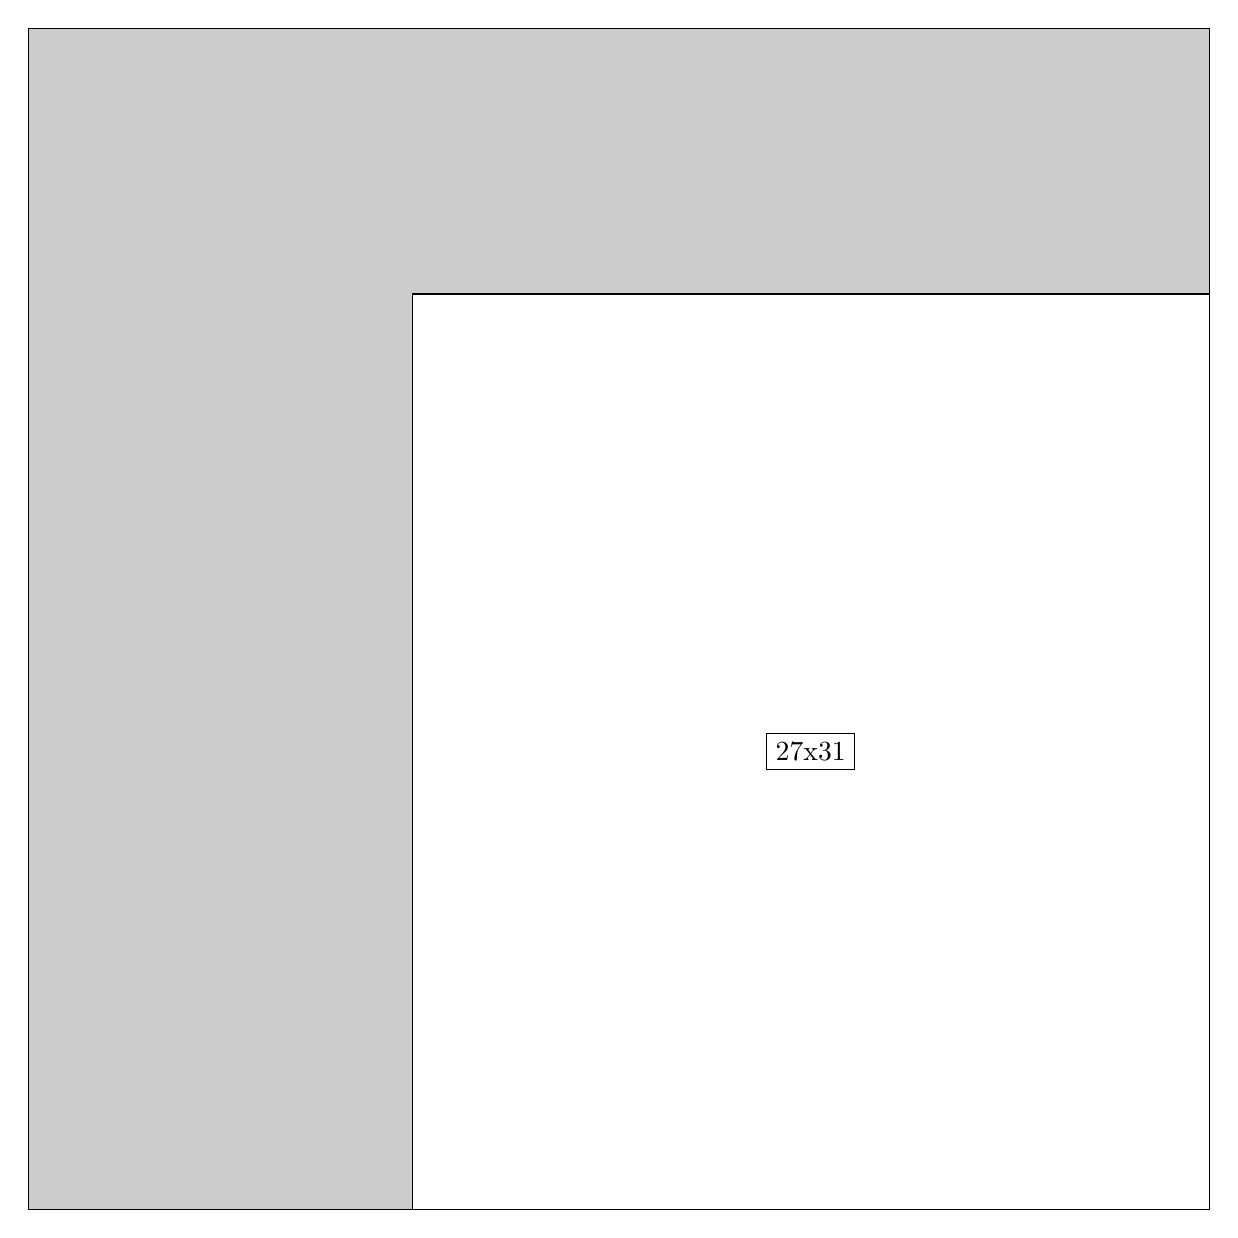
\begin{tikzpicture}[shorten >=1pt,scale=1.0,every node/.style={scale=1.0},->]
\tikzstyle{vertex}=[circle,fill=black!25,minimum size=14pt,inner sep=0pt]
\filldraw[fill=gray!40!white, draw=black] (0,0) rectangle (15.0,15.0);
\foreach \name/\x/\y/\w/\h in {27x31/4.875/0.0/10.125/11.625}
\filldraw[fill=white!40!white, draw=black] (\x,\y) rectangle node[draw] (\name) {\name} ++(\w,\h);
\end{tikzpicture}


w =27 , h =31 , x =13 , y =0 , v =837
\par
\newpage


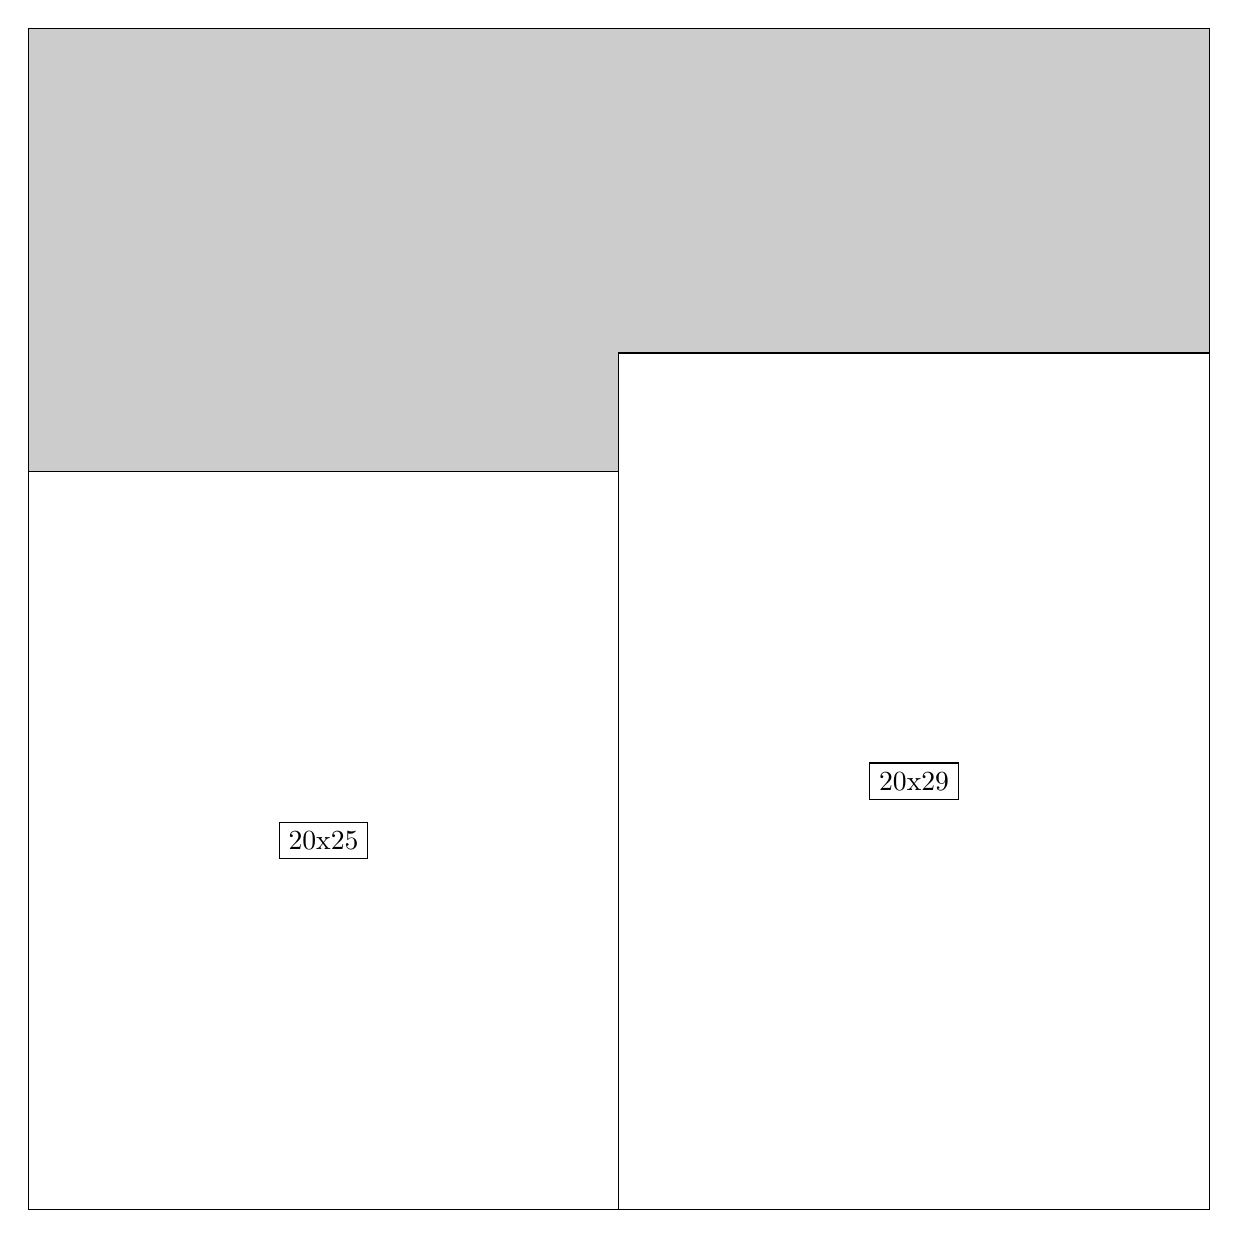
\begin{tikzpicture}[shorten >=1pt,scale=1.0,every node/.style={scale=1.0},->]
\tikzstyle{vertex}=[circle,fill=black!25,minimum size=14pt,inner sep=0pt]
\filldraw[fill=gray!40!white, draw=black] (0,0) rectangle (15.0,15.0);
\foreach \name/\x/\y/\w/\h in {20x29/7.5/0.0/7.5/10.875,20x25/0.0/0.0/7.5/9.375}
\filldraw[fill=white!40!white, draw=black] (\x,\y) rectangle node[draw] (\name) {\name} ++(\w,\h);
\end{tikzpicture}


w =20 , h =29 , x =20 , y =0 , v =580
\par
w =20 , h =25 , x =0 , y =0 , v =500
\par
\newpage


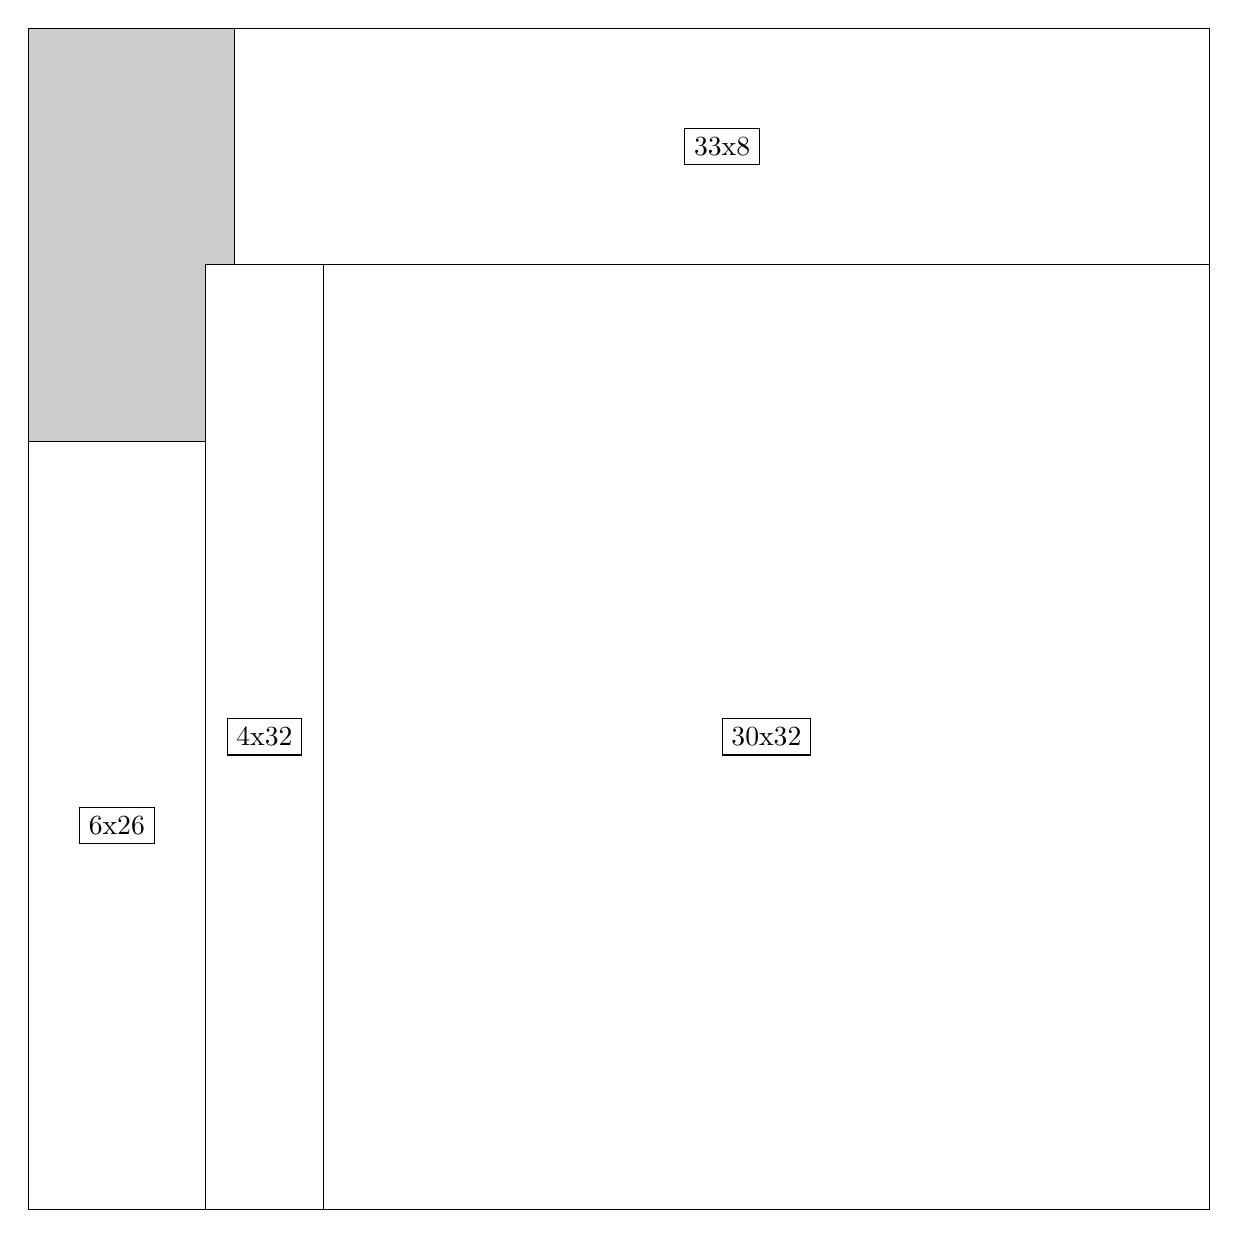
\begin{tikzpicture}[shorten >=1pt,scale=1.0,every node/.style={scale=1.0},->]
\tikzstyle{vertex}=[circle,fill=black!25,minimum size=14pt,inner sep=0pt]
\filldraw[fill=gray!40!white, draw=black] (0,0) rectangle (15.0,15.0);
\foreach \name/\x/\y/\w/\h in {30x32/3.75/0.0/11.25/12.0,4x32/2.25/0.0/1.5/12.0,6x26/0.0/0.0/2.25/9.75,33x8/2.625/12.0/12.375/3.0}
\filldraw[fill=white!40!white, draw=black] (\x,\y) rectangle node[draw] (\name) {\name} ++(\w,\h);
\end{tikzpicture}


w =30 , h =32 , x =10 , y =0 , v =960
\par
w =4 , h =32 , x =6 , y =0 , v =128
\par
w =6 , h =26 , x =0 , y =0 , v =156
\par
w =33 , h =8 , x =7 , y =32 , v =264
\par
\newpage


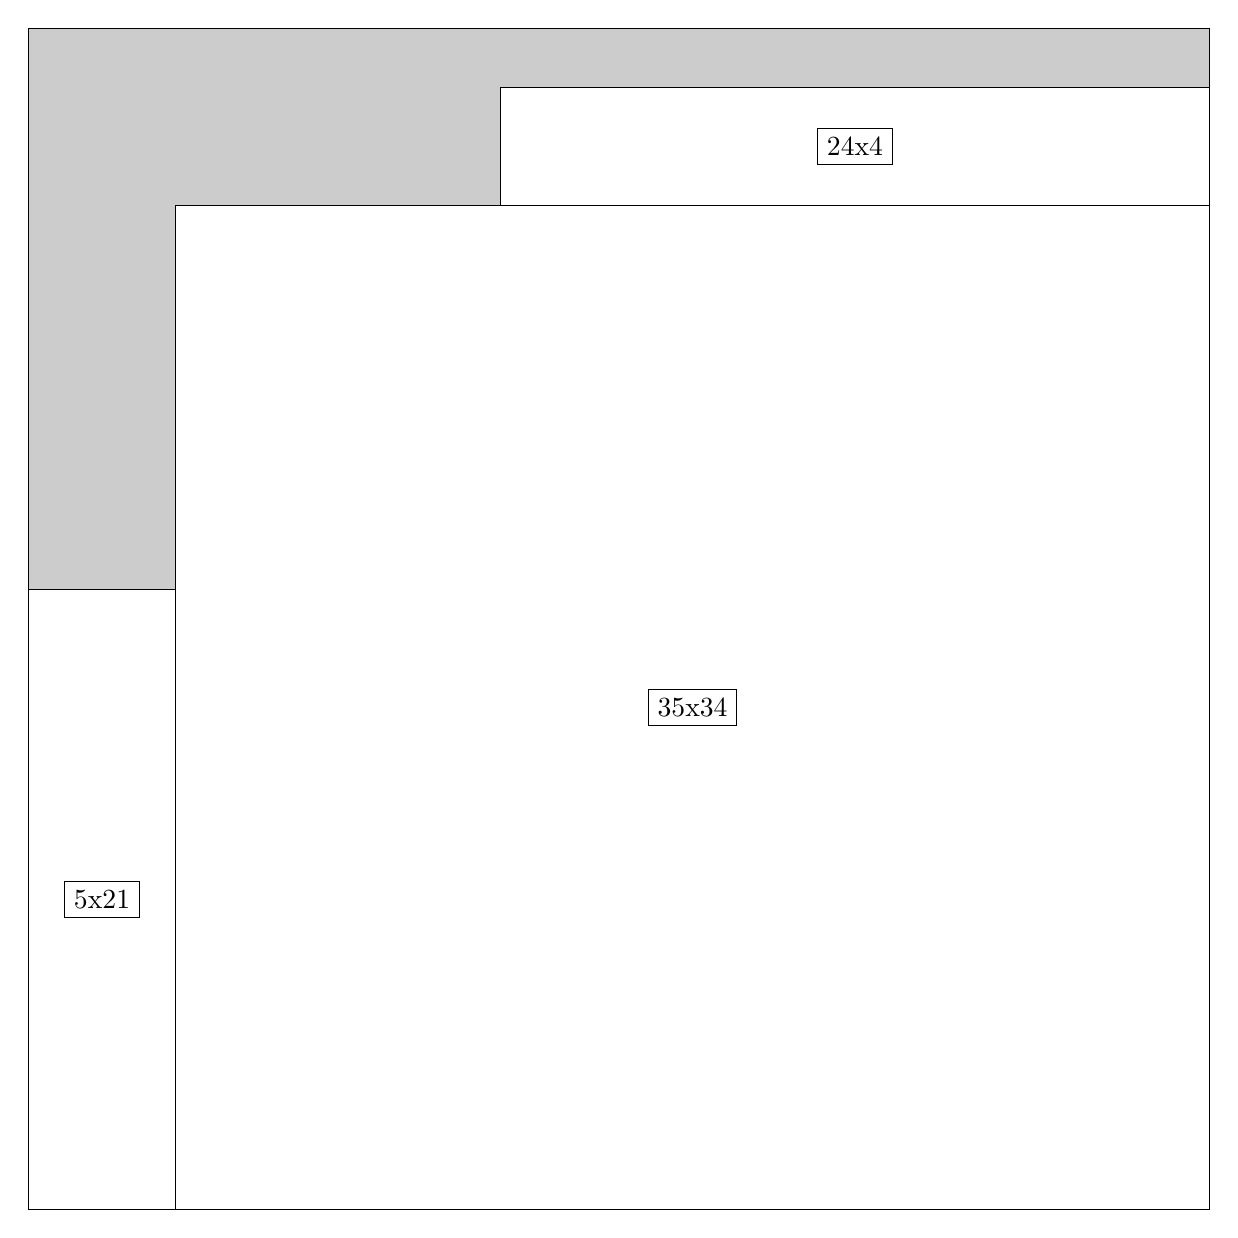
\begin{tikzpicture}[shorten >=1pt,scale=1.0,every node/.style={scale=1.0},->]
\tikzstyle{vertex}=[circle,fill=black!25,minimum size=14pt,inner sep=0pt]
\filldraw[fill=gray!40!white, draw=black] (0,0) rectangle (15.0,15.0);
\foreach \name/\x/\y/\w/\h in {35x34/1.875/0.0/13.125/12.75,5x21/0.0/0.0/1.875/7.875,24x4/6.0/12.75/9.0/1.5}
\filldraw[fill=white!40!white, draw=black] (\x,\y) rectangle node[draw] (\name) {\name} ++(\w,\h);
\end{tikzpicture}


w =35 , h =34 , x =5 , y =0 , v =1190
\par
w =5 , h =21 , x =0 , y =0 , v =105
\par
w =24 , h =4 , x =16 , y =34 , v =96
\par
\newpage


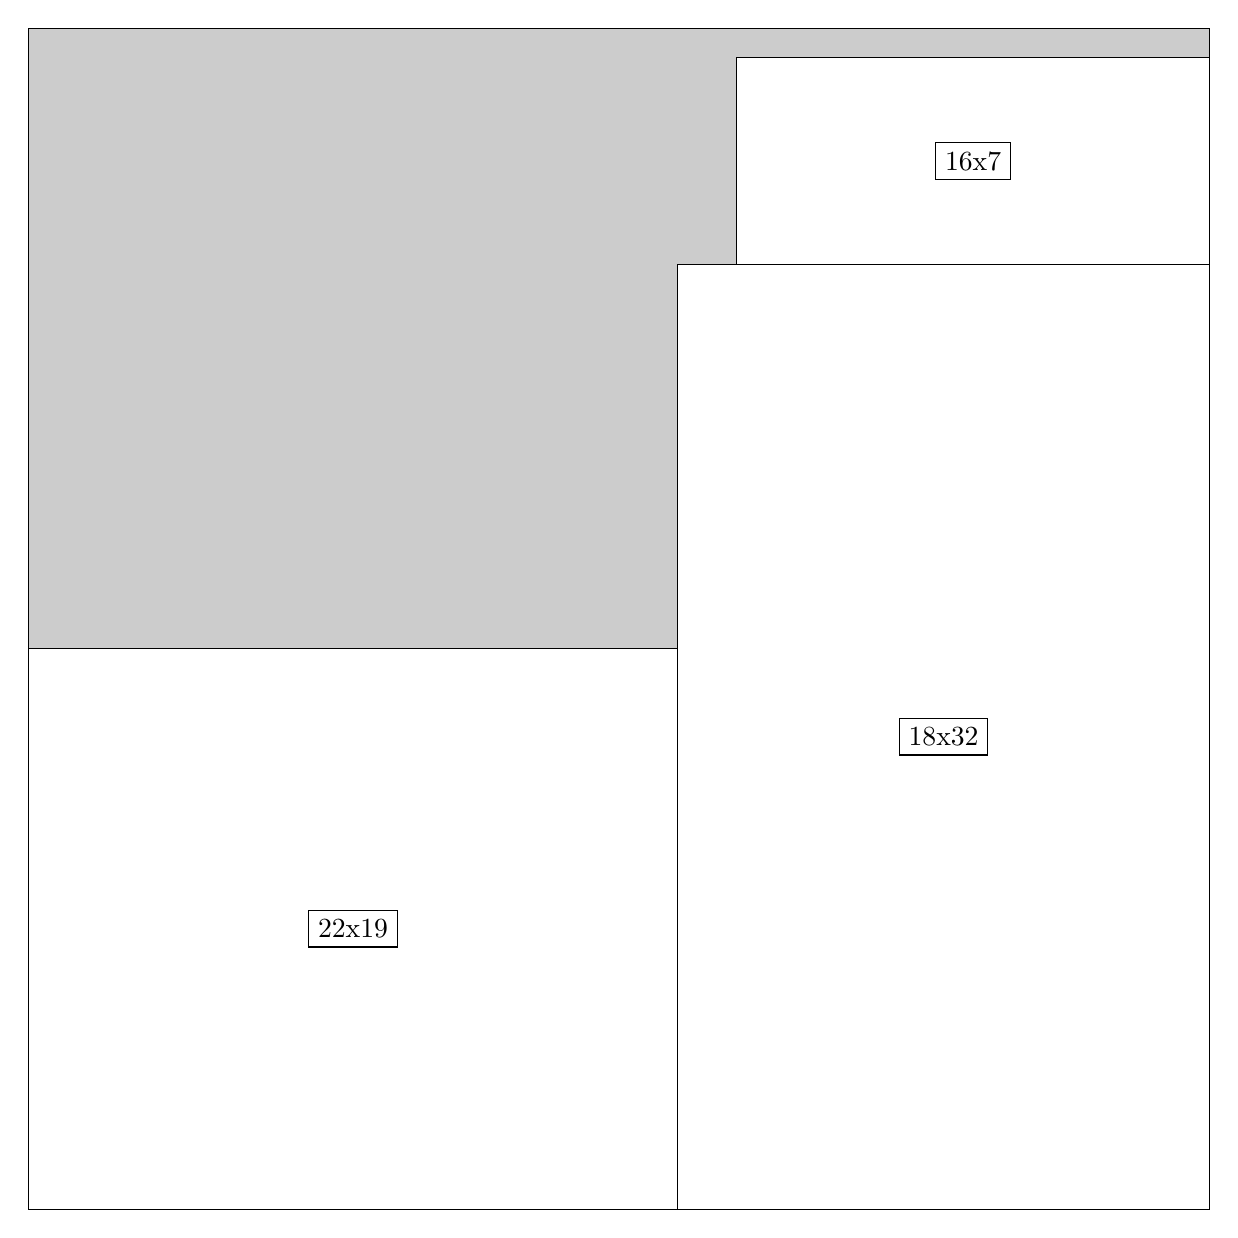
\begin{tikzpicture}[shorten >=1pt,scale=1.0,every node/.style={scale=1.0},->]
\tikzstyle{vertex}=[circle,fill=black!25,minimum size=14pt,inner sep=0pt]
\filldraw[fill=gray!40!white, draw=black] (0,0) rectangle (15.0,15.0);
\foreach \name/\x/\y/\w/\h in {18x32/8.25/0.0/6.75/12.0,16x7/9.0/12.0/6.0/2.625,22x19/0.0/0.0/8.25/7.125}
\filldraw[fill=white!40!white, draw=black] (\x,\y) rectangle node[draw] (\name) {\name} ++(\w,\h);
\end{tikzpicture}


w =18 , h =32 , x =22 , y =0 , v =576
\par
w =16 , h =7 , x =24 , y =32 , v =112
\par
w =22 , h =19 , x =0 , y =0 , v =418
\par
\newpage


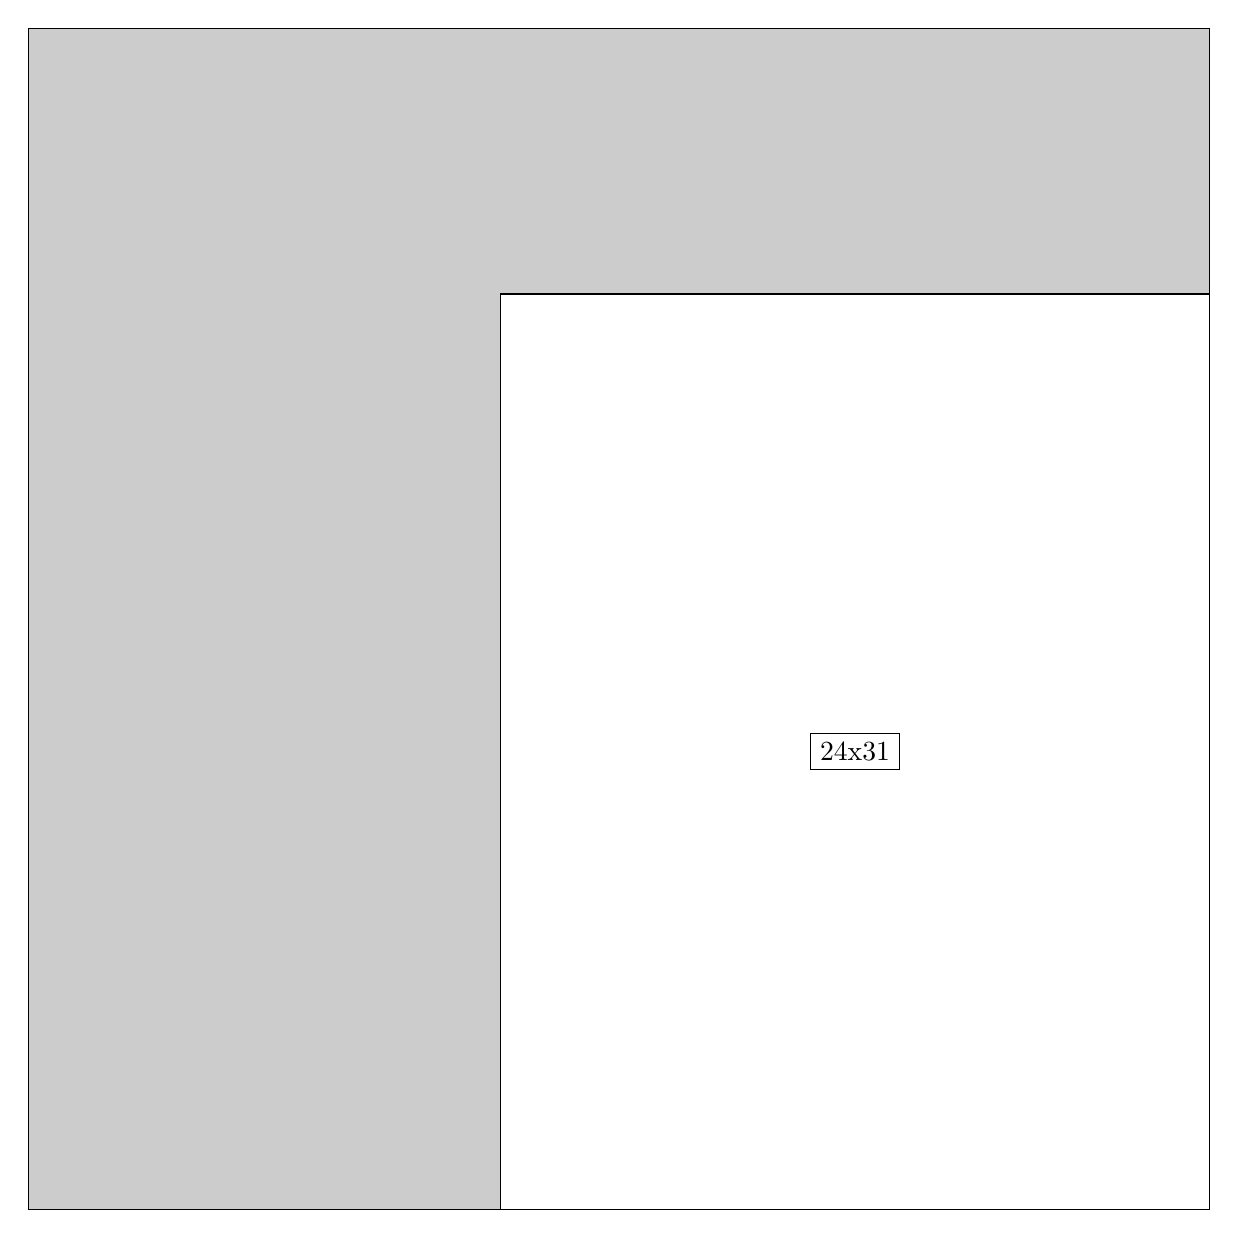
\begin{tikzpicture}[shorten >=1pt,scale=1.0,every node/.style={scale=1.0},->]
\tikzstyle{vertex}=[circle,fill=black!25,minimum size=14pt,inner sep=0pt]
\filldraw[fill=gray!40!white, draw=black] (0,0) rectangle (15.0,15.0);
\foreach \name/\x/\y/\w/\h in {24x31/6.0/0.0/9.0/11.625}
\filldraw[fill=white!40!white, draw=black] (\x,\y) rectangle node[draw] (\name) {\name} ++(\w,\h);
\end{tikzpicture}


w =24 , h =31 , x =16 , y =0 , v =744
\par
\newpage


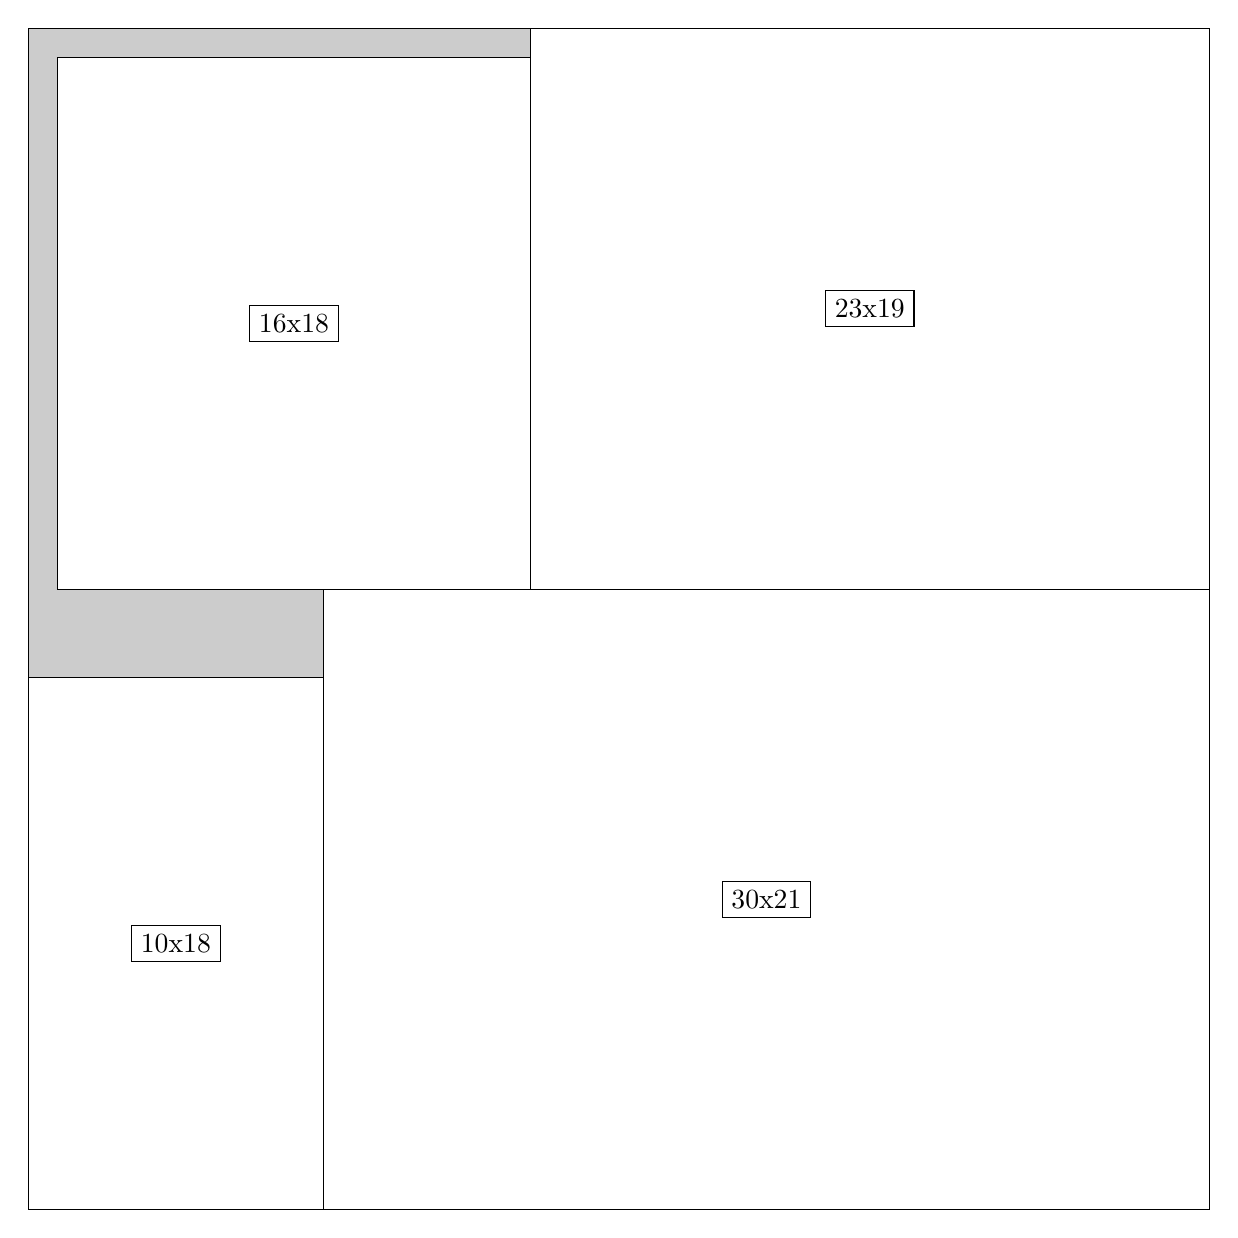
\begin{tikzpicture}[shorten >=1pt,scale=1.0,every node/.style={scale=1.0},->]
\tikzstyle{vertex}=[circle,fill=black!25,minimum size=14pt,inner sep=0pt]
\filldraw[fill=gray!40!white, draw=black] (0,0) rectangle (15.0,15.0);
\foreach \name/\x/\y/\w/\h in {30x21/3.75/0.0/11.25/7.875,10x18/0.0/0.0/3.75/6.75,23x19/6.375/7.875/8.625/7.125,16x18/0.375/7.875/6.0/6.75}
\filldraw[fill=white!40!white, draw=black] (\x,\y) rectangle node[draw] (\name) {\name} ++(\w,\h);
\end{tikzpicture}


w =30 , h =21 , x =10 , y =0 , v =630
\par
w =10 , h =18 , x =0 , y =0 , v =180
\par
w =23 , h =19 , x =17 , y =21 , v =437
\par
w =16 , h =18 , x =1 , y =21 , v =288
\par
\newpage


\end{document}